% !TeX spellcheck = en_US
% !TeX encoding = utf8
% !TeX program = xelatex
% !BIB program = biber 

% \documentclass{beamer}
\documentclass[usenames,dvipsnames,notes]{beamer}
% \documentclass[draft]{beamer}	
% \usetheme{Singapore}
% \usetheme{Hannover}
\usepackage{pgfpages}
\setbeameroption{hide notes} % Only slides
%\setbeameroption{show only notes} % Only notes
% \setbeameroption{show notes on second screen=right} % Both

\usepackage[british]{babel}
\usepackage{graphicx,hyperref,url, booktabs}
% \usepackage{ru}
\usepackage{math}
% \usepackage{hanging}
\usepackage{listings}
\usefonttheme[onlymath]{serif}
\usepackage{fontspec,xunicode}
% \setmainfont{Tahoma}
\usepackage[slantfont,boldfont]{xeCJK}
\setmainfont{Times New Roman}%缺省英文字体.serif是有衬线字体sans serif无衬线字体
\setCJKmainfont[ItalicFont={Adobe Kaiti Std}, BoldFont={Adobe Heiti Std}]{Adobe Song Std}%衬线字体 缺省中文字体为 %STSong

\pgfdeclareimage[width=\paperwidth,height=\paperheight]{bg}{background}
\setbeamertemplate{background}{\pgfuseimage{bg}}

\usepackage{animate}
% \usepackage[round]{natbib}
% \bibliographystyle{plainnat}
% \bibliographystyle{apalike} 
% \usepackage[backend=biber]{biblatex}
\usepackage{biblatex}

\bibliography{./ref.bib}
\addbibresource{ref.bib}
\usepackage{multirow}
\usepackage{booktabs}
\usepackage{indentfirst}
\usepackage{longtable}
\usepackage{float}
% \usepackage{picins}
\usepackage{rotating}
\usepackage{subfigure}
\usepackage{tabu}
\usepackage{amsmath}
\usepackage{amssymb}
\usepackage{setspace}
\usepackage{amsfonts}
\usepackage{appendix}
\usepackage{listings}
\usepackage{xcolor}
%\usepackage[colorlinks=true,
%pdfstartview=FitH,%
%linkcolor=blue,anchorcolor=violet,citecolor=magenta
%]{hyperref}
% \usepackage[dvipsnames]{xcolor}
\usepackage{geometry}

%%-----------------------xeCJK下设置中文字体------------------------------%
\newcommand{\verylarge}{\fontsize{60pt}{\baselineskip}\selectfont}  
\newcommand{\chuhao}{\fontsize{44.9pt}{\baselineskip}\selectfont}  
\newcommand{\xiaochu}{\fontsize{38.5pt}{\baselineskip}\selectfont}  
\newcommand{\yihao}{\fontsize{27.8pt}{\baselineskip}\selectfont}  
\newcommand{\xiaoyi}{\fontsize{25.7pt}{\baselineskip}\selectfont}  
\newcommand{\erhao}{\fontsize{23.5pt}{\baselineskip}\selectfont}  
\newcommand{\xiaoerhao}{\fontsize{19.3pt}{\baselineskip}\selectfont} 
\newcommand{\sihao}{\fontsize{14pt}{\baselineskip}\selectfont}      % 字号设置  
\newcommand{\xiaosihao}{\fontsize{12pt}{\baselineskip}\selectfont}  % 字号设置  
\newcommand{\wuhao}{\fontsize{10.5pt}{\baselineskip}\selectfont}    % 字号设置  
\newcommand{\xiaowuhao}{\fontsize{9pt}{\baselineskip}\selectfont}   % 字号设置  
\newcommand{\liuhao}{\fontsize{7.875pt}{\baselineskip}\selectfont}  % 字号设置  
\newcommand{\qihao}{\fontsize{5.25pt}{\baselineskip}\selectfont}    % 字号设置 

\graphicspath{{./fig/}}

% \setbeamertemplate{footnote}{%
%   \hangpara{2em}{1}%
%   \makebox[2em][l]{\insertfootnotemark}\footnotesize\insertfootnotetext\par%
% }

\definecolor{cred}{rgb}{0.6,0,0}
\definecolor{cgreen}{rgb}{0.25,0.5,0.35}
\definecolor{cpurple}{rgb}{0.5,0,0.35}
\definecolor{cdocblue}{rgb}{0.25,0.35,0.75}
\definecolor{cdark}{rgb}{0.95,1.0,1.0}
\lstset{
	language=python,
	numbers=left,
	numberstyle=\tiny\color{black},
	keywordstyle=\color{cpurple},
	commentstyle=\color{cgreen},
	stringstyle=\color{cred},
	% frame=single,
	% escapeinside=``,
	% xleftmargin=1em,
	% xrightmargin=1em, 
	backgroundcolor=\color{cdark},
	% aboveskip=1em,
	% breaklines=true,
	% tabsize=3
} 

\makeatletter
\long\def\beamer@author[#1]#2{%
  \def\insertauthor{\def\inst{\beamer@insttitle}\def\and{\beamer@andtitle}%
  \begin{tabular}{rl}#2\end{tabular}}%
  \def\beamer@shortauthor{#1}%
  \ifbeamer@autopdfinfo%
    \def\beamer@andstripped{}%
    \beamer@stripands#1 \and\relax
    {\let\inst=\@gobble\let\thanks=\@gobble\def\and{: }\hypersetup{pdfauthor={\beamer@andstripped}}}
  \fi%
}
\makeatother

% \setbeamersize{text margin left=60mm} 
\setbeamertemplate{frametitle}[default][right]

% The title of the presentation:
%  - first a short version which is visible at the bottom of each slide;
%  - second the full title shown on the title slide;
\title[毕设答辩]{\bf 毕业论文答辩}

% Optional: a subtitle to be dispalyed on the title slide
\subtitle{\it 深度行人再识别学习}

% The author(s) of the presentation:
%  - again first a short version to be displayed at the bottom;
%  - next the full list of authors, which may include contact information;
\author[xinglu]{
	姓名学号: & 王兴路 3140102282 \\
	% 指导老师: & 李英明 \\
	年级专业: & 2014级信息工程
}
% The institute:
%  - to start the name of the university as displayed on the top of each slide
%    this can be adjusted such that you can also create a Dutch version
%  - next the institute information as displayed on the title slide

% \institute[信工1403]{}

% Add a date and possibly the name of the event to the slides
%  - again first a short version to be shown at the bottom of each slide
%  - second the full date and event name for the title slide
\date[\today]{2018年6月5日}

\begin{document}

\AtBeginSection[]
{
	\begin{frame}
		\frametitle{大纲}
		\tableofcontents[currentsection]
	\end{frame}
}

% \AtBeginSubsection[2-]
% {
%    \begin{frame}
%        \frametitle{大纲}
%        \tableofcontents[currentsection]
%    \end{frame}
% }

\begin{frame}
	\titlepage
	\note{2018/06/01--2018/06/08毕业论文答辩。老师们同学们好,很高心能参加这次毕设答辩,我的毕设题目是深度行人再识别学习
		我将分三步介绍我的毕设,背景、方案和思考}
\end{frame}

% \begin{frame}{Embedded Animation}
%   \animategraphics[loop,controls,width=.6\linewidth]{10}{stn-}{0}{52}
% \end{frame}

\section{背景介绍与研究内容}

\begin{frame}
	{背景介绍}
	\begin{itemize}
		\item 行人再识别在智能视频监控、智能安防邻域应用广泛
		\item 摄像机网络广泛布控于各种公共场合中,采集的数据具有{\bf 跨摄像头}的特性
		\item 摄像头采集了{\bf 海量}数据,需要智能分析技术快速检索
	\end{itemize}
	\begin{figure}
		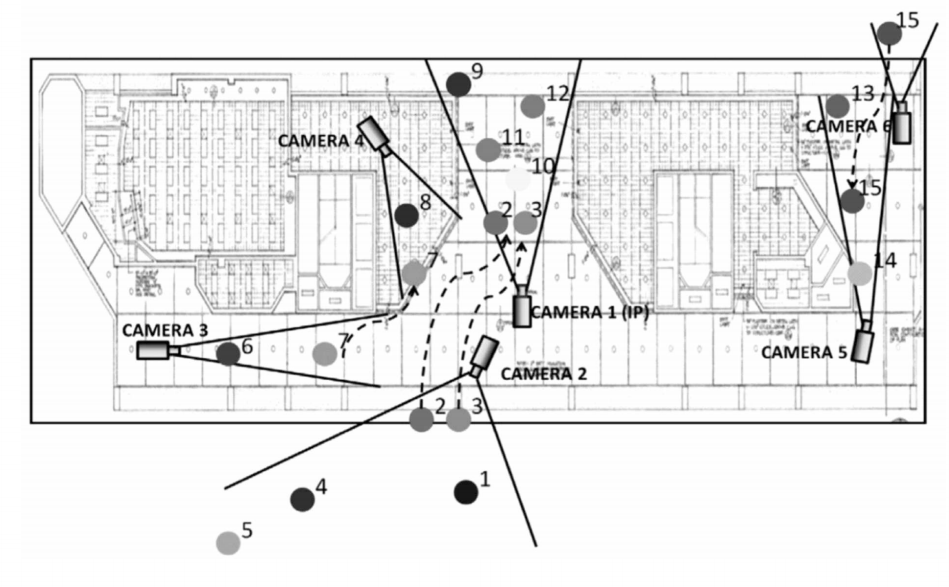
\includegraphics[width=0.75\linewidth]{2018-03-07-19-33-13.png}
	\end{figure}
	\note{
		我们有大规模的摄像头网络,有海量的数据,借此我们有可能完成更高层的任务,比如疑犯追踪,异常行为检测
		。但是面对多
		路监控和海量的视频数据,监控人员很容易 疲惫和应接不暇 ,因此我们需要智能分析技术 来完成海量的工作。
		于是想要最基础的任务,行人再识别应运而生。
	}
\end{frame}


\begin{frame}
	{行人再识别的定义}
	% \begin{block}
	\begin{itemize}
		\item 广义的行人再识别:行人检测 $\rightarrow$ 行人跟踪 $\rightarrow$ 行人检索
		\item 狭义的行人再识别\cite{zheng2016person}: 行人检索
	\end{itemize}
	% \end{block}
	\begin{figure}
		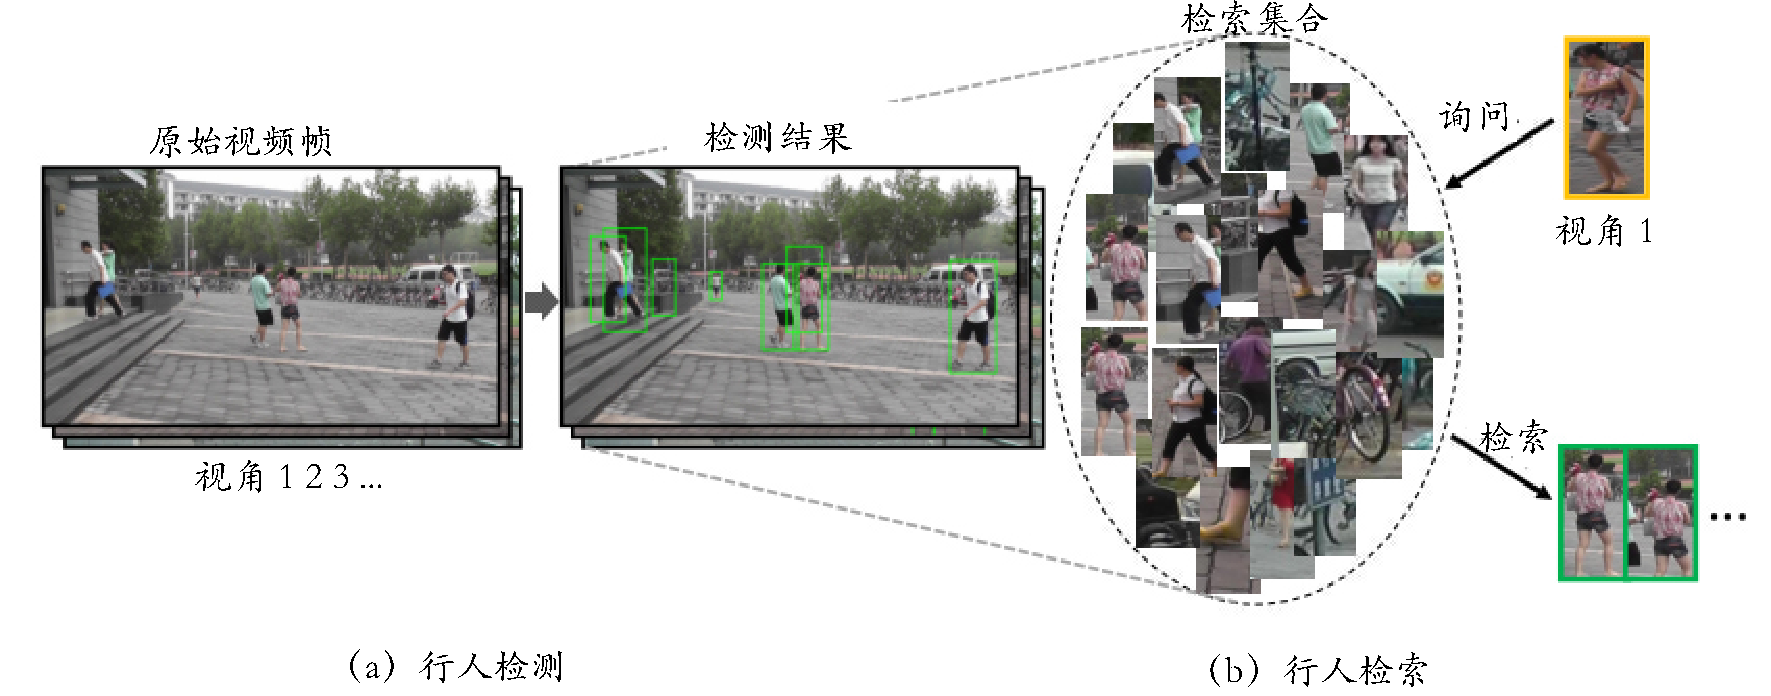
\includegraphics[width=1\linewidth]{fig/background.pdf}
	\end{figure}
	\note{
		行人再识别有广义和狭义之分,目前
		学术界研究行人再识别的论文都采用狭义的定义,
		也就是行人再识别
		建立在检测好的图片的基础上
		我们也不列外,研究行人检索问题。
	}
\end{frame}

\begin{frame}
	{行人再识别定义}
	\begin{block}{行人再识别 (Person Re-identification,  ReID)}
		输入某一行人的询问图片(probe), 在检索集合(gallery)中{\bf 跨摄像头}检索所有包含该行人的图片。
	\end{block}
	\begin{columns}
		\column{0.3\textwidth}
		\centering
		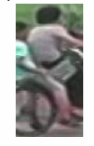
\includegraphics[width=0.5\linewidth]{2018-03-12-10-05-13.png} \\
		\it 询问图
		\column{0.7\textwidth}
		\centering
		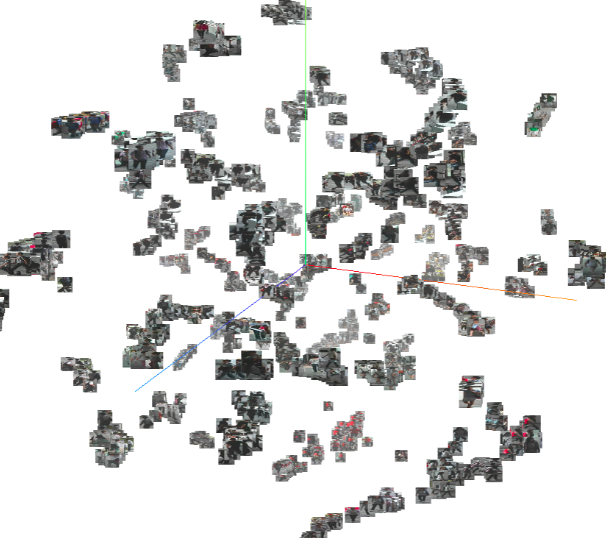
\includegraphics[width=0.72\linewidth]{2018-03-12-09-57-11.png} \\
		\it 检索集合
	\end{columns}
	\note{
		行人再识别是图像检索的子问题 , 他是这样的一个过称:
		输入询问图片,如左图所示,在右图测试图像集合中寻找最为匹配的行人图片
		匹配是指达到两点要求:1 两幅图属于同一个人,2 跨摄像头
		与一般的图像检索的不同 就体现在 跨摄像头,也就是行人再识别存在着许多行人图片共享一个摄像头视角的情况。
	}
\end{frame}

\begin{frame}
	{行人再识别定义}
	\begin{block}{行人再识别 (Person Re-identification, ReID)}
		输入某一行人的询问图片(probe),在检索集合(gallery)中{\bf 跨摄像头}检索所有包含该行人的图片。
	\end{block}
	\begin{figure}
		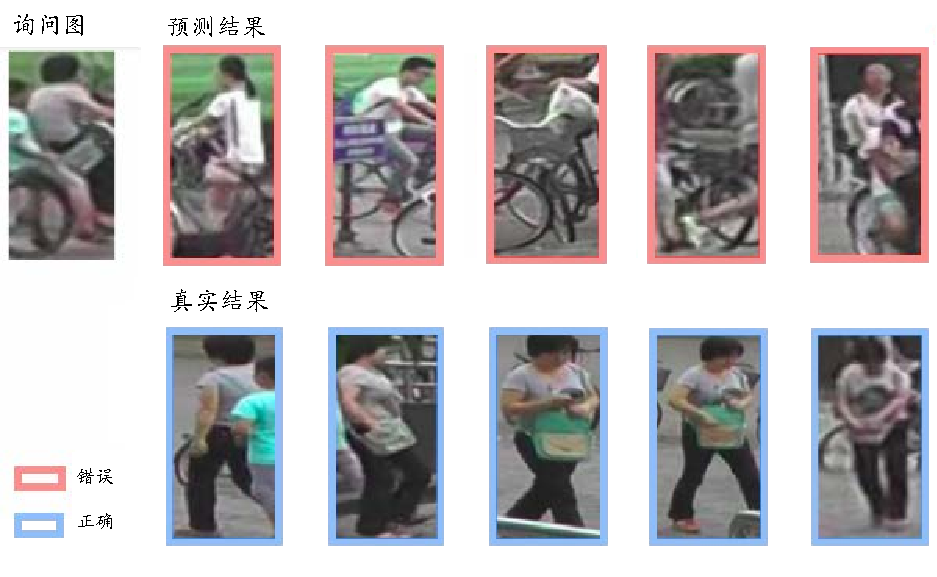
\includegraphics[width=0.9\linewidth]{2018-03-11-22-56-05.pdf}
	\end{figure}
	\note{
		举例而言,输入询问图片,我们的基准模型的预测结果如右侧所示,她是一个按照置信度排序的列表,右侧上方显示了模型认为最有可能的5张图片,下方为真实结果,由于草地、自行车、遮挡等干扰,模型没有一个预测争取。可见再识别任务十分困难。}
\end{frame}


\begin{frame}
	{存在的挑战}
	\begin{description}
		\item[遮挡] 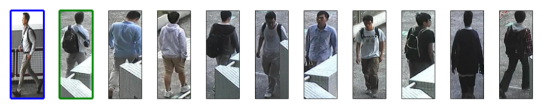
\includegraphics[width=0.9\linewidth]{2018-03-12-10-09-03.png}
		\item[光照变化] 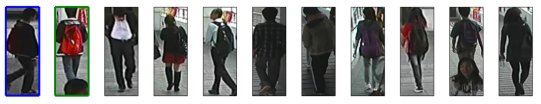
\includegraphics[width=0.9\linewidth]{2018-03-12-10-10-10.png}
		\item[姿态变化] 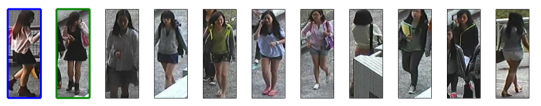
\includegraphics[width=0.9\linewidth]{2018-03-12-10-10-18.png}
		\item[空间失配] 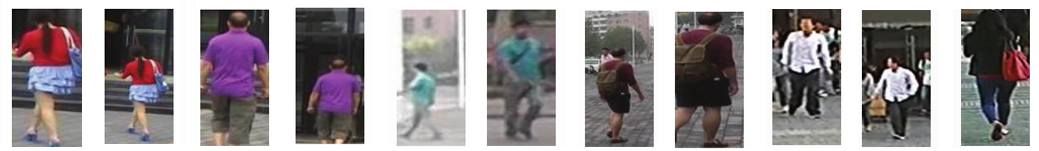
\includegraphics[width=0.88\linewidth]{2018-03-07-20-16-25.png}
	\end{description}

	\note{
		再识别的面临的挑战包括 遮挡、明暗、姿态倒置的行人外观巨大改变,以及由于检测器误差导致的空间适配。
	}
\end{frame}

\begin{frame}
	{研究内容}
	\begin{itemize}
		\item 检测器误差 $\Rightarrow$ 空间失配
		\item 摄像机视角差异 $\Rightarrow$ 行人姿态变化
	\end{itemize}
\end{frame}

\section{技术路线与设计方案}

\subsection{基于注意力机制的多尺度特征融合}

\begin{frame}{动机}
	空间失配导致的失败案例:
	\begin{figure}
		\centering
		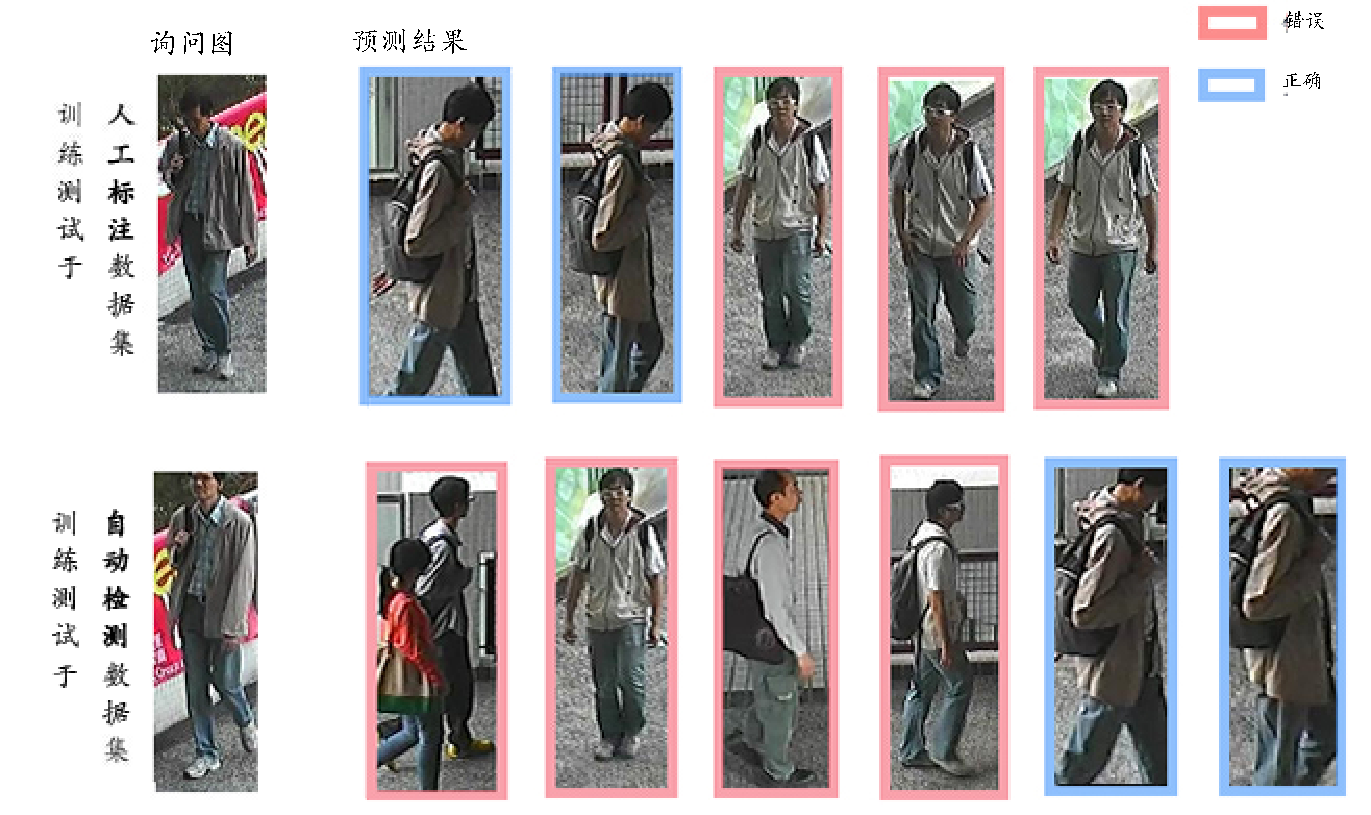
\includegraphics[width=\textwidth]{fig/2018-04-18-21-53-15.pdf}
		% \caption{我们的基准模型在手工标注的数据集和行人检测器自动检测的数据集上的典型样例} 
		\label{fig:label2det}
	\end{figure}
	\note{
		面对空间失配,我们采用
		基于注意力机制的多尺度特征融合。
		它的动机是来源于对数据集的观察。
		在做研究的阶段,我们会同时有人工标注好的数据和检测器自动检测的数据。两者的不同如图所示,自动检测数据不是截取了行人的头部和脚步,就是引入了干扰的行人。
		我们在两个数据集上使用相同结构的模型验证,发现在自动检测数据集上训练的结果较为不理想。
		于是我们打算这样解决问题,
		首先,除去整体是相似性,模型应当关注一些局部的相似性,从而在失配情况下,能够根据一些局部语义部件匹配成功。
		其次,对于低层属性特征,我们要有选择地提取,比如我们会表述行人的衣服颜色属性为灰色,而背景的红色颜色属性或者干扰行人的红色属性应当去除。
	}
\end{frame}

\begin{frame}{基准模型}
	Qian Yu \etal 提出多尺度融合\cite{yu2017devil}:
	\begin{figure}
		\centering
		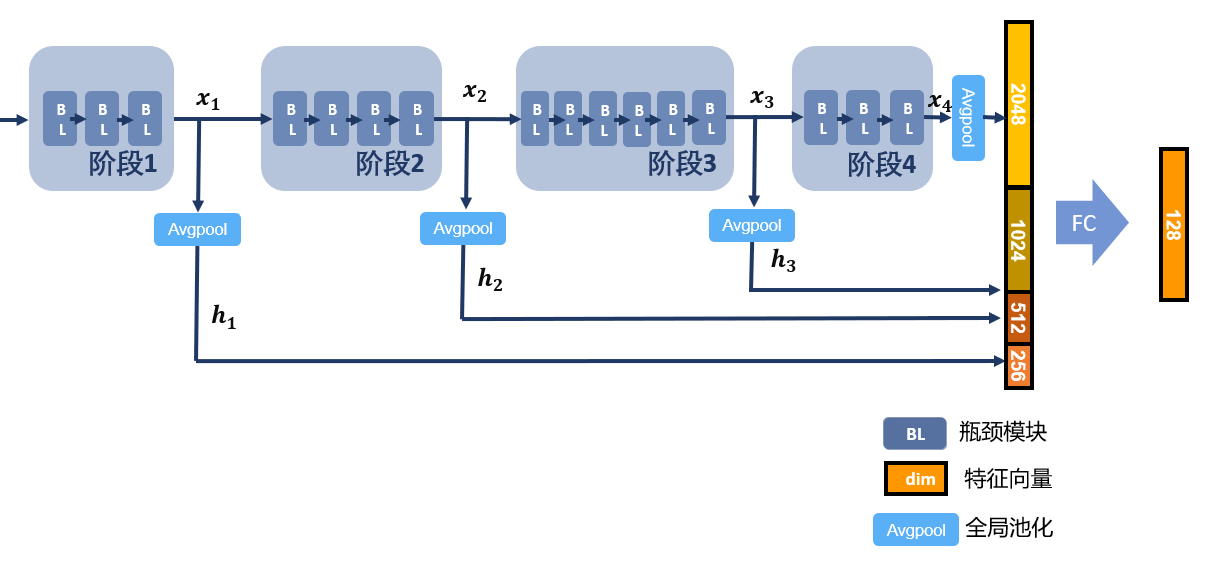
\includegraphics[width=.92\textwidth]{fig/baseline.png}
		% \caption{中层特征与全局特征的融合方式}
		\label{fig:fusion}
	\end{figure}
	\note{
		低层属性特征与全局语义特征融合
		多分别率
		想要融入低层属性特征,我们很容易想到将残差网络的每个阶段的特征拼合在一起。我们之后的工作在此基础上改进。
		目前,我们仍然没有实现有选择地提取属性特征和提取语义部件的功能。
	}
\end{frame}

\begin{frame}{提取属性特征和语义部件}
	采用注意力机制,考虑各种注意力机制的合理性:
	\begin{columns}
		\column{.3\textwidth}
		空间变换 \\
		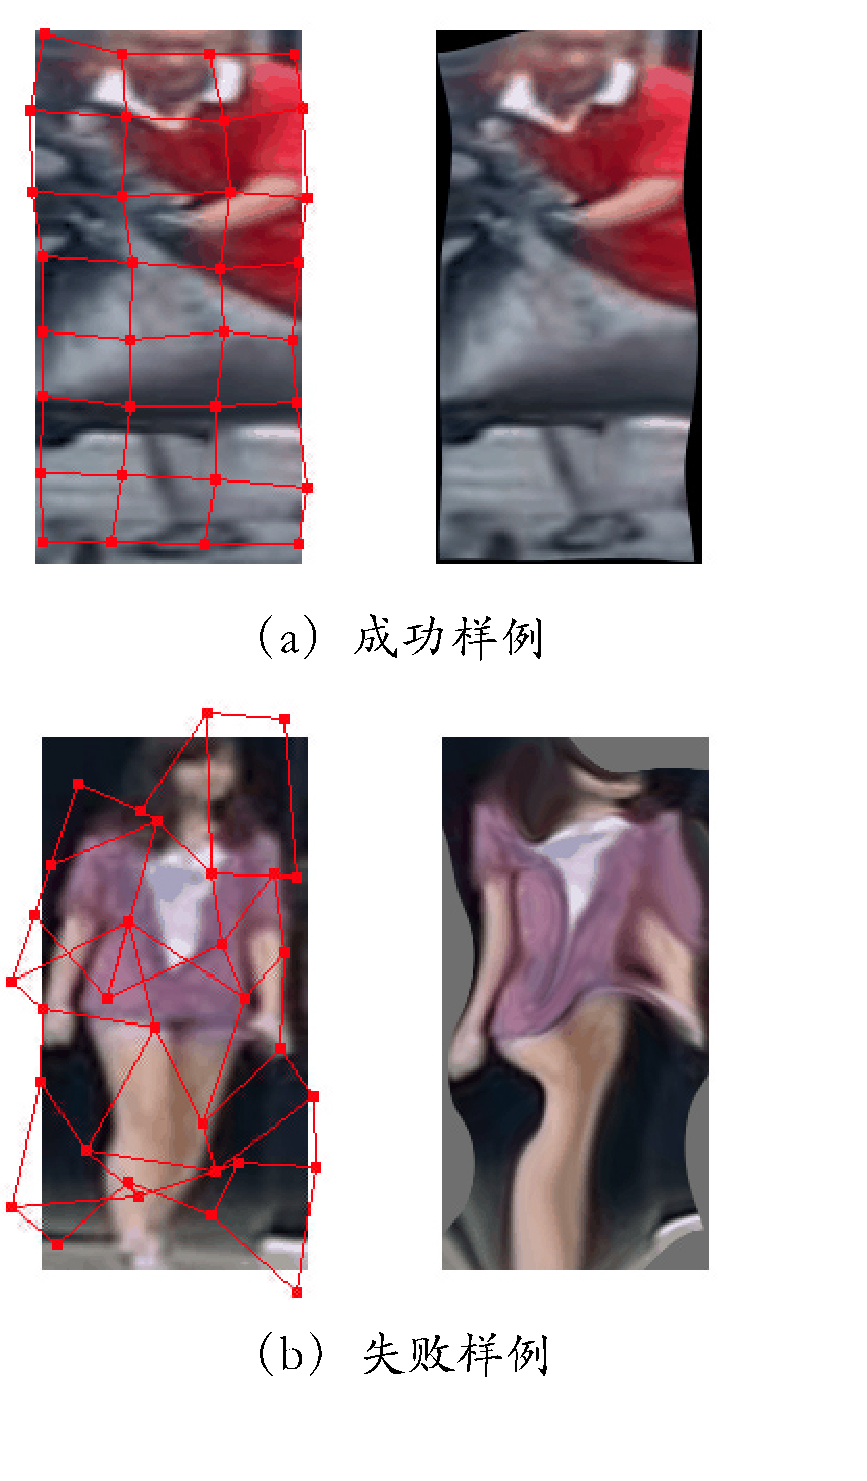
\includegraphics[width=\textwidth]{fig/stn.pdf}

		\column{.7\textwidth}
		空间级别 \\
		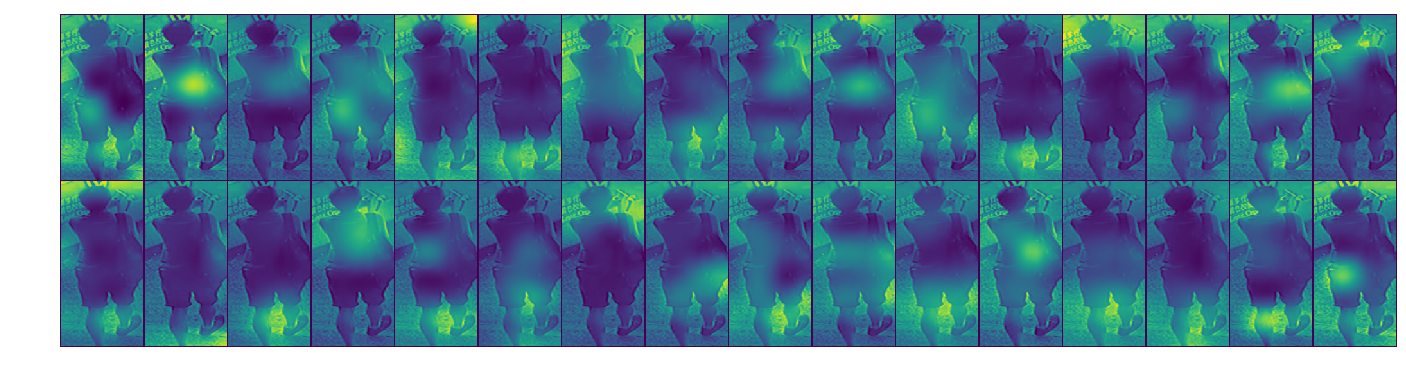
\includegraphics[width=\textwidth]{fig/spatial.png}
		通道级别 \\
		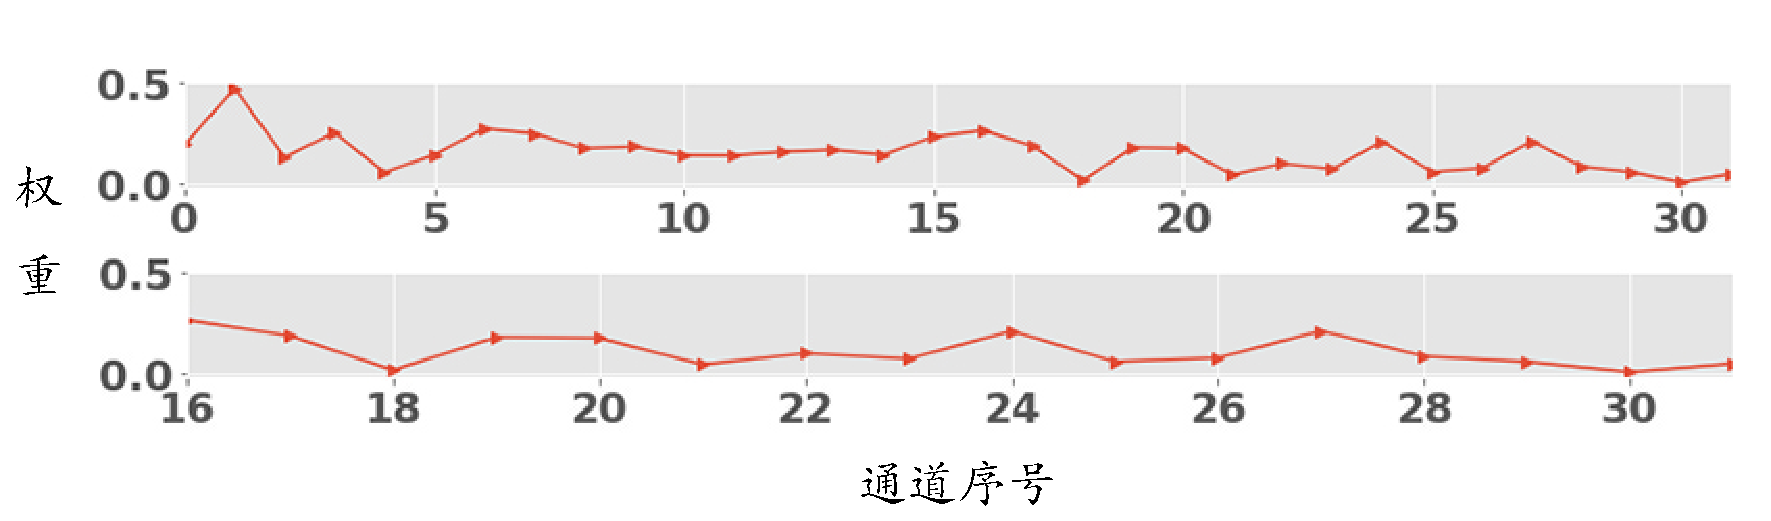
\includegraphics[width=\textwidth]{fig/chnl.pdf}

	\end{columns}
	%	 \begin{itemize}
	%	 	\item 空间级别: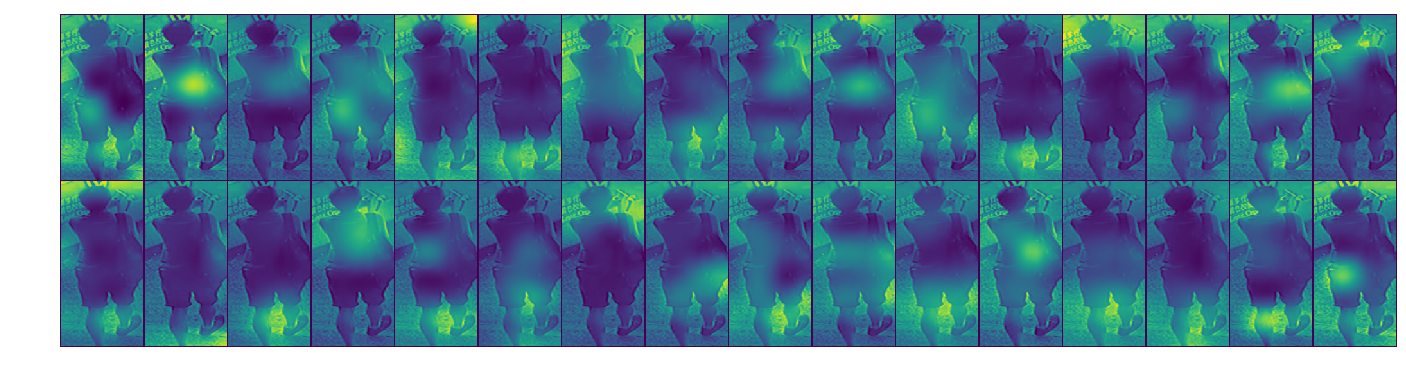
\includegraphics[width=.5\textwidth]{fig/spatial.png}
	%	 	\item 通道级别: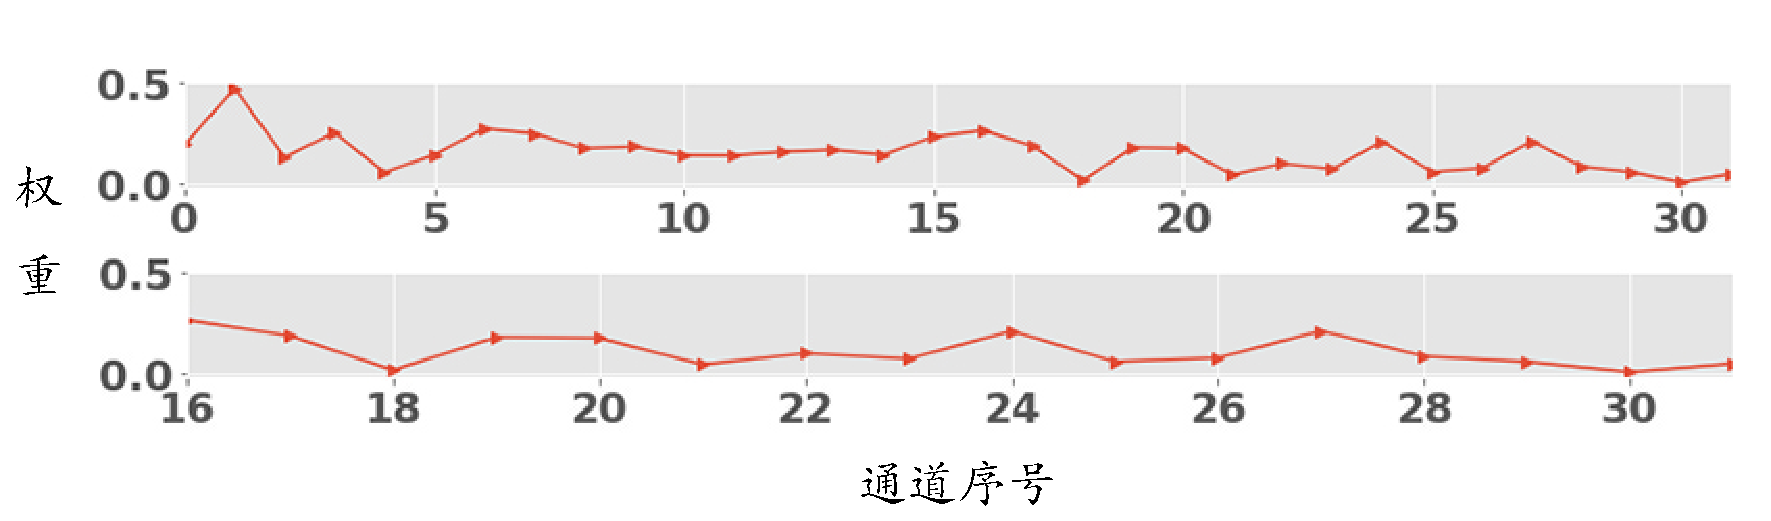
\includegraphics[width=.5\textwidth]{fig/chnl.pdf}
	%	 	\item 空间变换: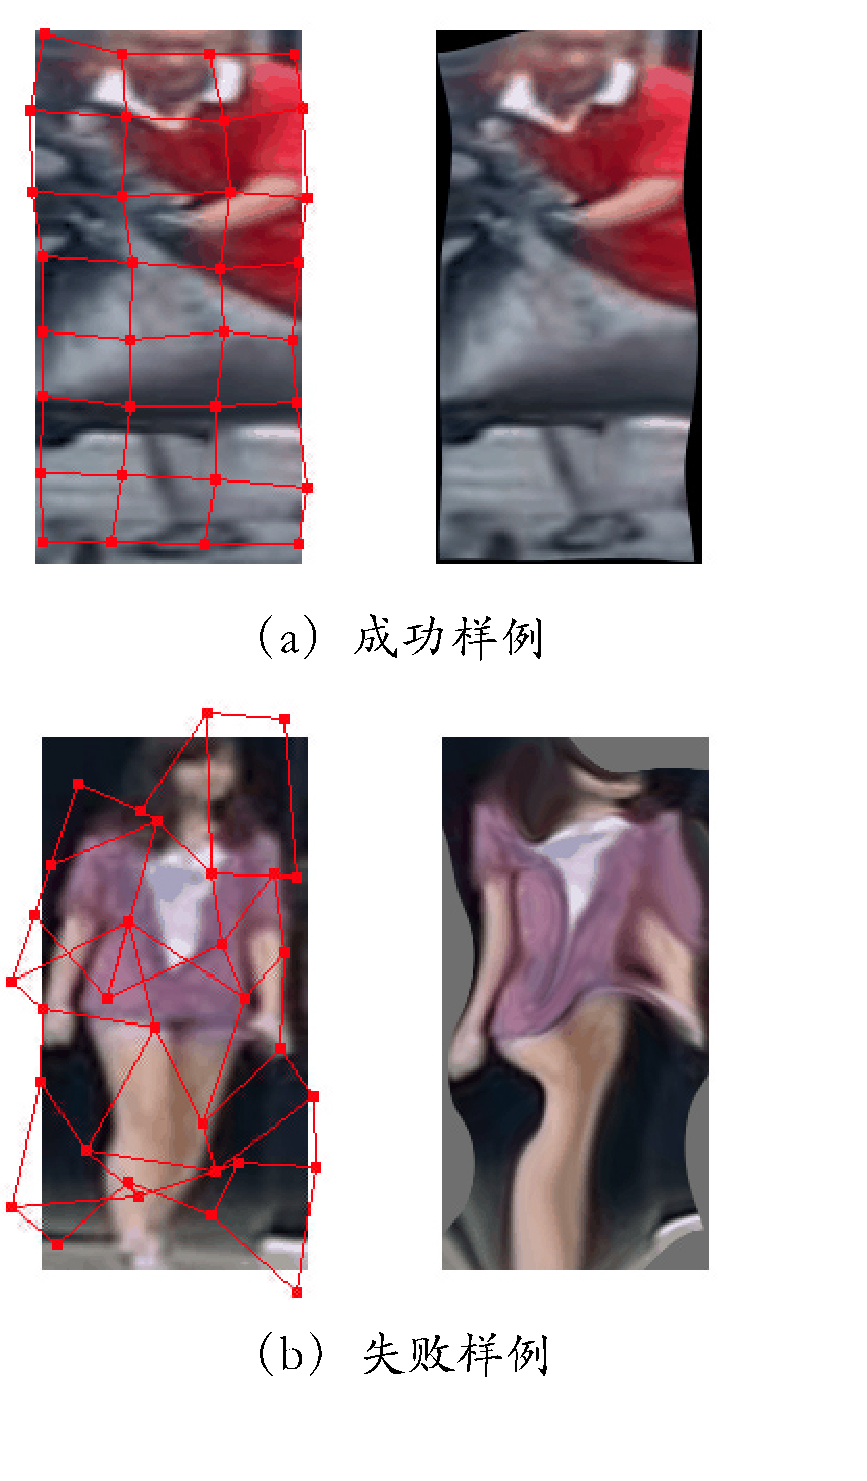
\includegraphics[width=.5\textwidth]{fig/stn.pdf}
	%	 \end{itemize}
	\note{首先看一下空间变换,它希望通过对图片进行重采样来学习对旋转平移缩放形变都鲁棒的特征。但是目前看到的实现,都需要特别的技巧比如恒等初始化、恒等正则化、学习率降十倍等技巧稳定,所以就暂时没有使用。接下来我们会分析为什么空间级别的注意力不太合理,以及为什么最终采用了通道级别的注意力。}
\end{frame}

\begin{frame}{空间级别注意力}
	输入一个视角的行人图片:
	\begin{columns}
		\column{.1\textwidth}
		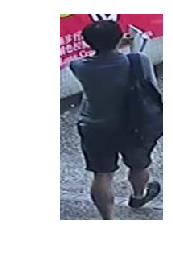
\includegraphics[width=\textwidth]{fig/ori-ped.png}
		\column{.9\textwidth}
		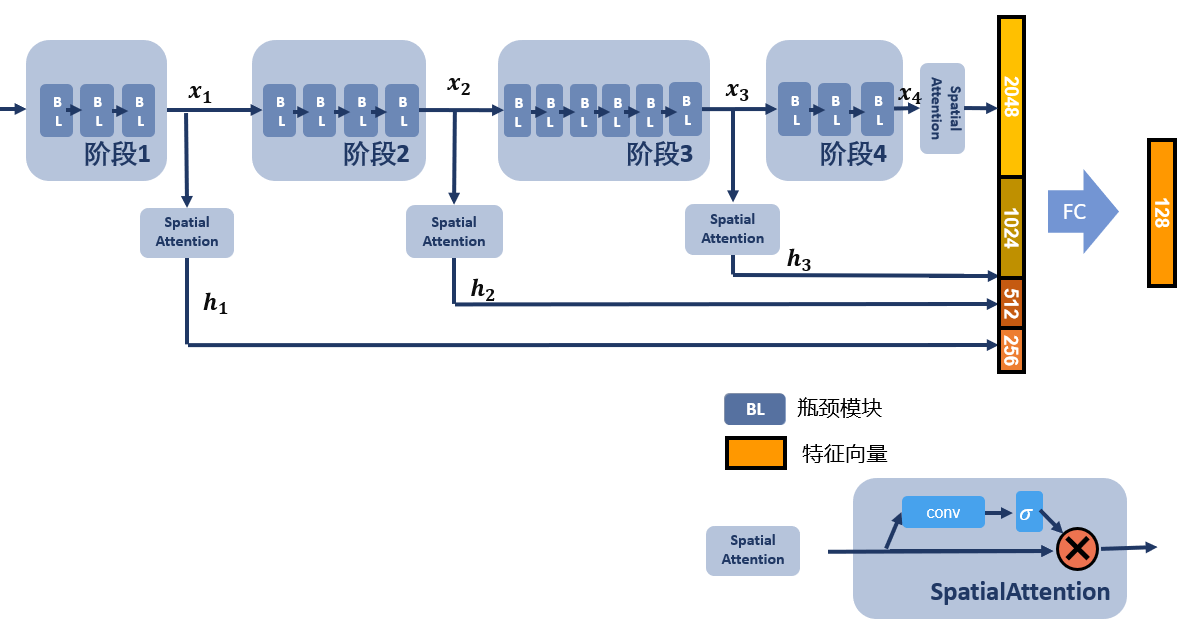
\includegraphics[width=\textwidth]{fig/spatial-att.png}
	\end{columns}
	\note{
		空间级别的注意力对特征进行如图所示的变换,
		输入一个视角的行人图片,观察阶段一和阶段四的重(spatial mask—)z注意力权重
	}
\end{frame}

\begin{frame}{空间级别注意力}
	阶段一的注意力权重(spatial mask)为:\\
	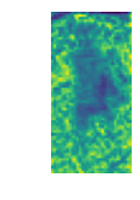
\includegraphics[height=.3\textheight]{fig/spatial-high-mask.png} 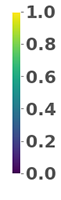
\includegraphics[height=.3\textheight]{fig/colorbar.png} \\
	阶段四的注意力权重为:\\
	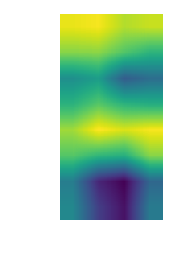
\includegraphics[height=.3\textheight]{fig/spatial-low-mask.png} 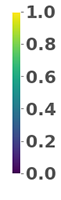
\includegraphics[height=.3\textheight]{fig/colorbar.png} \\
	其中,第四阶段注意力权重立方差值上采样为输入图像分辨率。
	\note{
		图中分别是第一和第四阶段的注意力权重,亮色代表权重数字较高,深色蓝色表示数值较低。
		现在看起来似乎有一定合理,但是。。。
	}
\end{frame}

\begin{frame}{空间级别注意力}
	阶段一的注意力权将应用在特征图的所有通道上:\\
	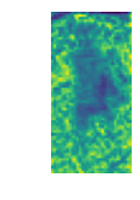
\includegraphics[height=.15\textheight]{fig/spatial-high-mask.png} 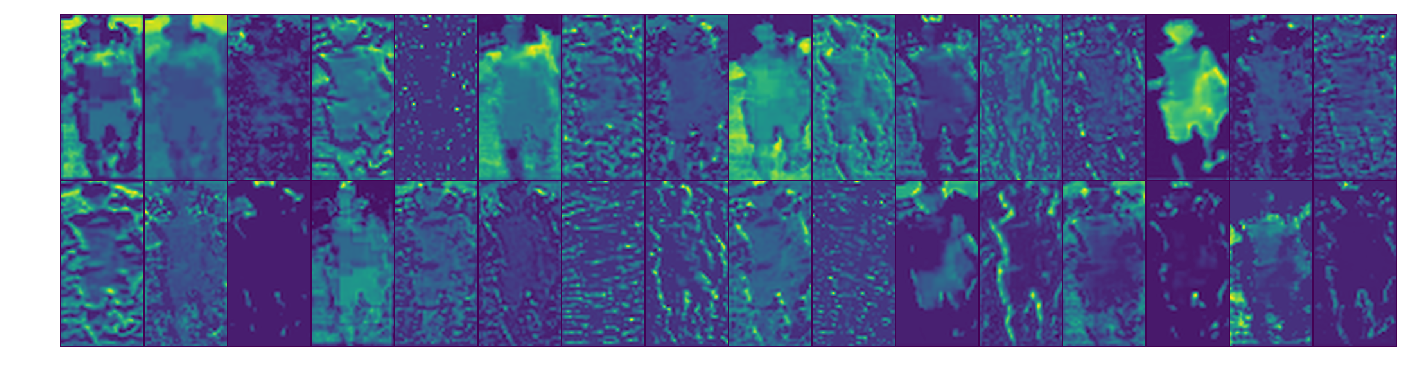
\includegraphics[height=.26\textheight]{fig/spatial-low.png} \\
	阶段四的注意力权重将应用在特征图的所有通道上:\\
	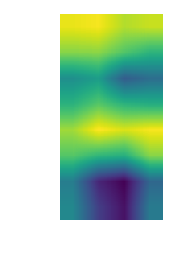
\includegraphics[height=.15\textheight]{fig/spatial-low-mask.png} 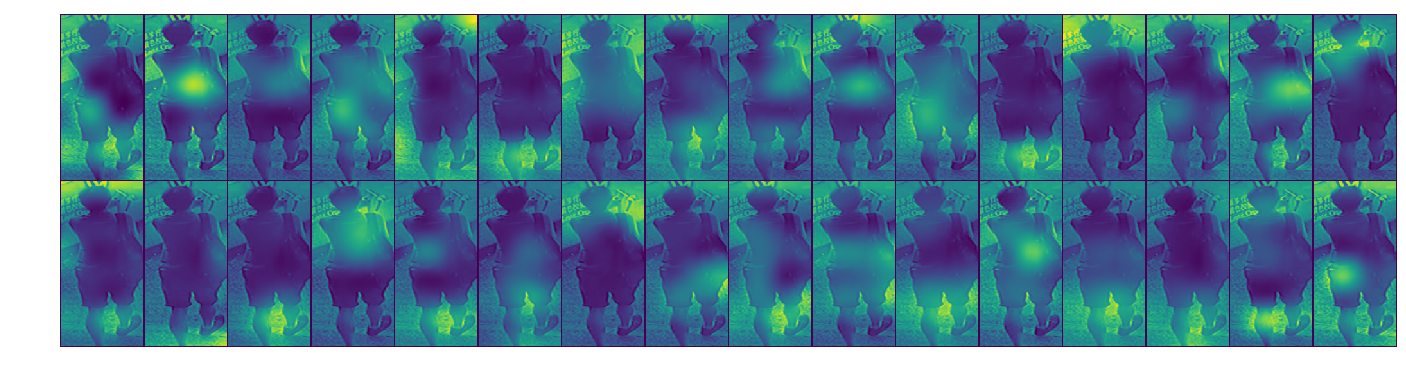
\includegraphics[height=.26\textheight]{fig/spatial.png} \\
	其中,为方便观察注意力所在的语义部件,阶段四的特征图与原图混合(blend)显示。
	\note{我们知道卷积层的特征图为三维张量,也就是一个注意力权重会应用到不同的通道上,不管通道编码了什么样的信息。对于低层特征有的通道也许是文理属性,有的是颜色属性;对于高层特征,也许是不同的人体部分。对所有通道采用相同权重显然不合理。近期分工作有一些采用多分支生成多个注意力权重,分组使用的方法。但是都增加了很多计算量和参数数量。}
\end{frame}


\begin{frame}{通道级别注意力}
	有选择地提取属性特征
	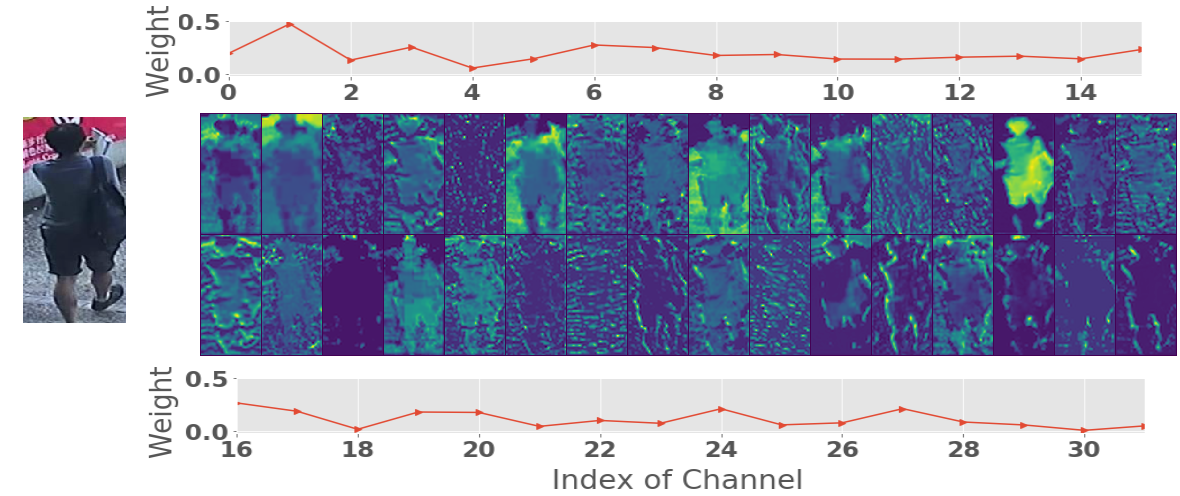
\includegraphics[width=\textwidth]{fig/comb0.png}
	\note{通道级别的注意力会更为合理,
先直接看一下他的效果,他确实可以
		 有选择地提取属性特征}
\end{frame}

\begin{frame}{通道级别注意力}
	提取语义部件
	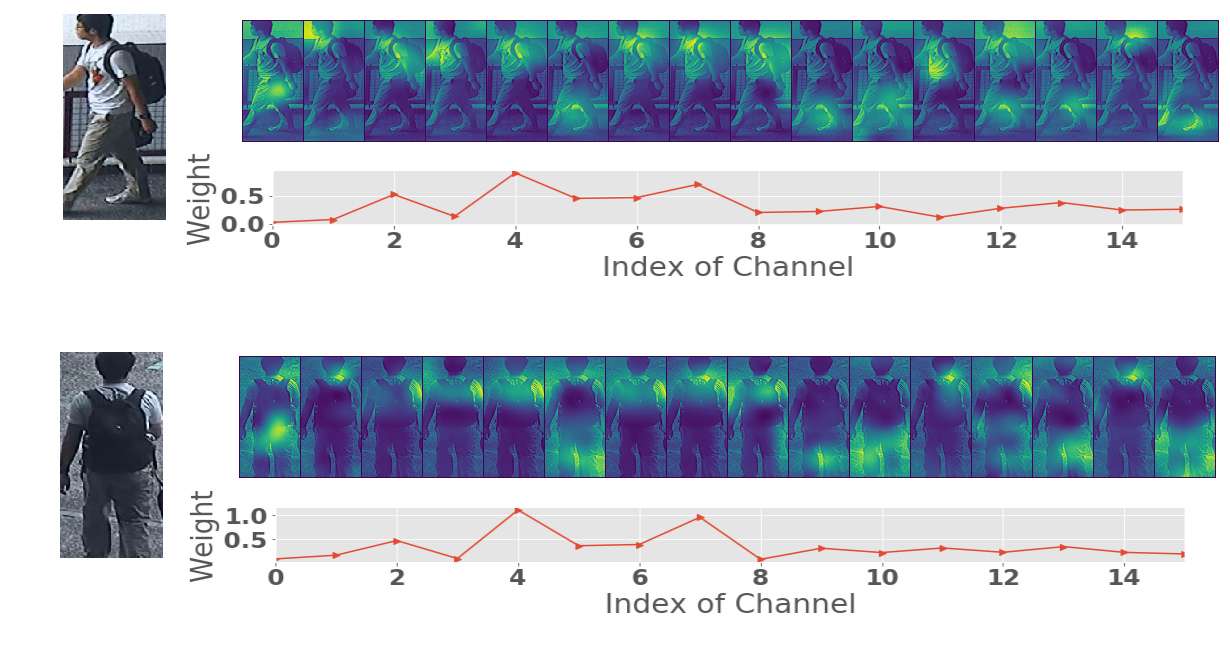
\includegraphics[width=\textwidth]{fig/comb1.png}
	\note{
	对于高层语义特征
		不同通道编码不同特征,注意力机制来选择,更为合理。 	这里只是先大致看一下它的效果,之后实验的定性分析中还会在提到,}
\end{frame}


\begin{frame}{方案:空间注意力+多尺度融合}
	提取局部属性特征:
	\begin{figure}
		\centering
		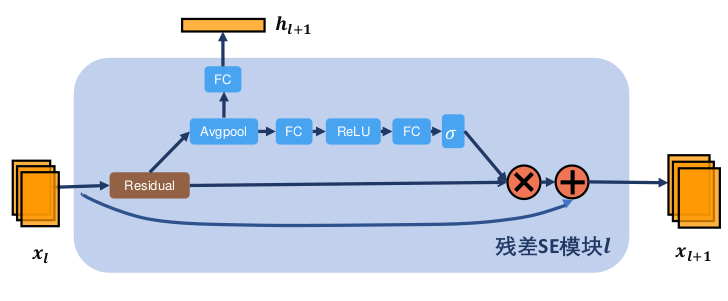
\includegraphics[width=.7\textwidth]{fig/2018-05-11-16-53-10.png}
		% \caption{兼具提取属性特征作用的残差SE模块}
		\label{fig:resse}
	\end{figure}
	多尺度融合:
	\begin{figure}
		\centering
		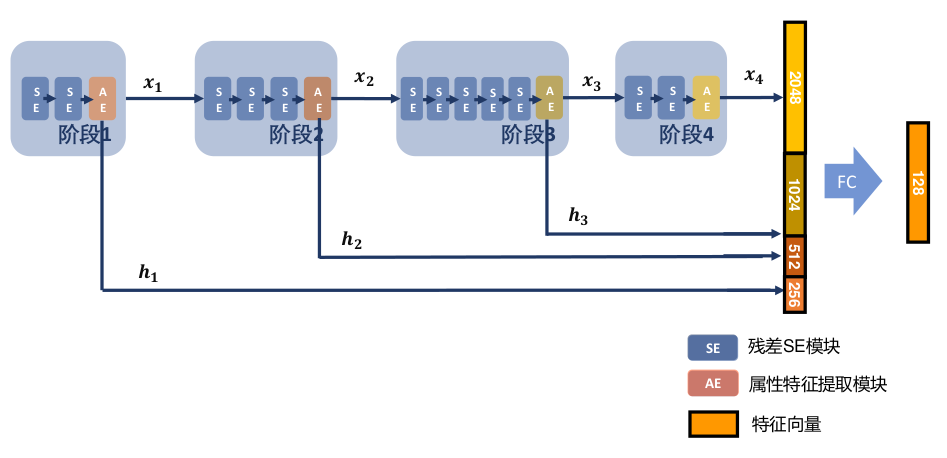
\includegraphics[width=.92\textwidth]{fig/2018-05-11-16-54-07.png}
		% \caption{中层特征与全局特征的融合方式}

	\end{figure}
	\note{对于通道级别的注意力我们也不是简单地加一个通道注意力模块的,
		我们采用se形式的注意力机制,
	
	通过实验和交叉验证,
			我们发现阶段属性特征与特征重标定权重(特征)不能共享, 
			最后一阶段注意力权重呈现均匀分布,为进步一减少计算量的增加,最后一阶段的注意力模块被去除。

		我们设计的结构。
		是注意力机制和多尺度融合的有机结合,

	}
\end{frame}


\begin{frame}{通道级别注意力}
	\begin{figure}
		\centering
		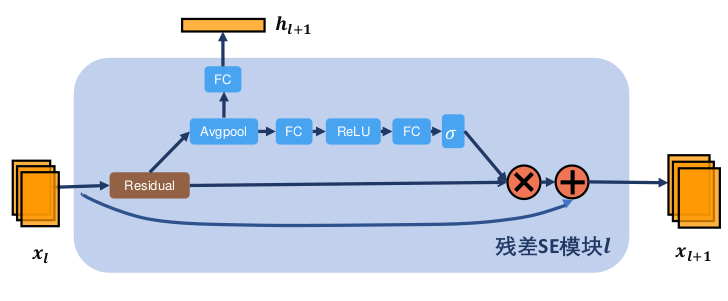
\includegraphics[width=.7\textwidth]{fig/2018-05-11-16-53-10.png}
		% \caption{兼具提取属性特征作用的残差SE模块
	\end{figure}
	\begin{itemize}
		\item 有选择地提取属性特征  {\liuhao:舍弃背景/无意义的属性特征,组合生成新的特征} 
		\item 提取语义部件 {\liuhao:高层特征的一个通道表示一个语义部件/抽象概念,选择有鉴别力的语义部件,从而避免空间失配的干扰} 
		\pause
		\item 与主流的分类网络兼容
		\item 基本不增加计算量和显存开销
		\item 输入相关的动态注意力机制
	\end{itemize}
	\note{
可以再任何		预训练的好的模型上插入我们的模块进一步提升
			我们设计的多功能的注意力模块, 由于 使用瓶颈结构自适应重标定通道特征,去除冗余特征,组合生成新的特征,获得解耦的表示。
			因而具有了期望的特性
			此外,我们还具有许多其他, 
			除去列出的还有,
		全局池化获得最大感受野,嵌入获得这一阶段特征表示。		 
		由于通道注意力的权重来自于特征图,因此这是一种动态的输入相关的注意力机制。		
	}
\end{frame}

\begin{frame}{实验}
	在数据集CUHK03上的CMC-1,CMC-5,CMC-10性能指标比对:
	\begin{table}
		\centering
		% \caption{在数据集CUHK03上的CMC-1,CMC-5,CMC-10性能指标比对}
		\scalebox{0.9}{
			\begin{tabular}{c|ccc|ccc}
				\hline
				\multirow{2}*{Methods}                     & \multicolumn{3}{c|}{labelled CUHK03} & \multicolumn{3}{c}{detected CUHK03}                                                              \\
				\cline{2-7} \cline{2-7}                    & r=1                                  & r=5                                 & r=10    & r=1                          & r=5     & r=10    \\ \hline
				KISSME \cite{kissme}                       & 14.17                                & 37.46                               & 52.20   & 11.70                        & 33.45   & 45.69   \\
				LMNN \cite{lmnn}                           & 7.29                                 & 19.64                               & 30.74   & 6.25                         & 17.87   & 26.60   \\
				LOMO+XQDA \cite{xqda}                      & 52.20                                & 82.23                               & 92.14   & 46.25                        & 78.90   & 88.55   \\ \hline
				ImprovedDL \cite{improveddl}               & 54.74                                & 86.50                               & 93.88   & 44.96                        & 76.01   & 81.85   \\
				DCSL (with hnm) \cite{yaqing2016semantics} & 80.20                                & 97.73                               & 99.17   & -                            & -       & -       \\
				JLML \cite{jlml}                           & 83.20                                & 98.00                               & 99.40   & 80.60                        & {96.90} & {98.70} \\
				SC-PPMN (with hnm) \cite{mao2018multi}     & {85.50}                              & {98.20}                             & {99.50} & {80.63}                      & 95.62   & 98.07   \\ \hline \hline
				TriHard Baseline                           & 84.91                                & 98.35                               & 99.24   & 81.88                        & 96.34   & 98.44   \\
				+ SE Attention                             & 87.03                                & 98.50                               & 99.18   & 83.50                        & 93.90   & 95.69   \\
				+ Multi-Scale Fusion                       & {\color{RoyalBlue}  88.28 }          & 98.44                               & 99.25   & {\color{NavyBlue} \bf 85.93} & 95.37   & 97.06   \\
				+ Rerank                                   & {\color{MidnightBlue} 96.34 }        & 99.24                               & 99.57   & 91.53                        & 98.32   & 98.95   \\ \hline
			\end{tabular}
		}
		\label{tab:cuhk03}
	\end{table}

\end{frame}

\begin{frame}{实验}
	在Market1501和DukeMTMC上的CMC-1, mAP性能指标对比:
	\begin{table}
		\centering
		% \caption{在数据集Market1501和DukeMTMC上的CMC-1, mAP性能指标对比}
		\label{tab:market}
		\begin{tabular}{c|cc|cc}
			\hline
			\multirow{2}*{Method}                & \multicolumn{2}{c|}{Market1501} & \multicolumn{2}{c}{DukeMTMC-ReID}                 \\
			\cline{2-5} \cline{2-5}              & r=1                             & mAP                               & r=1   & mAP   \\ \hline
			SomaNet                              & 73.87                           & 47.89                             & 76.70 & 56.80 \\
			PAN                                  & 82.81                           & 63.35                             & 71.59 & 51.51 \\
			TriHard in \cite{hermans2017defense} & 82.99                           & 66.63                             & 73.24 & 54.60 \\
			AWTL                                 & 84.20                           & 68.03                             & 74.23 & 54.97 \\ \hline  \hline
			TriHard Baseline                     & 84.62                           & 68.68                             & 76.32 & 59.57 \\
			+ SE Attention                       & 86.79                           & 70.61                             & 77.29 & 61.12 \\
			+ Multi-Scale Fusion                 & \blue{87.51}                    & 72.34                             & 77.12 & 61.64 \\
			+ Rerank                             & 89.19                           & 85.08                             & 79.39 & 72.57 \\ \hline
		\end{tabular}
	\end{table}
\note{传统方法
	
深度网络方法

基于注意力机制的多尺度融合}
\end{frame}

\begin{frame}{通道级别注意力}
	失配问题
	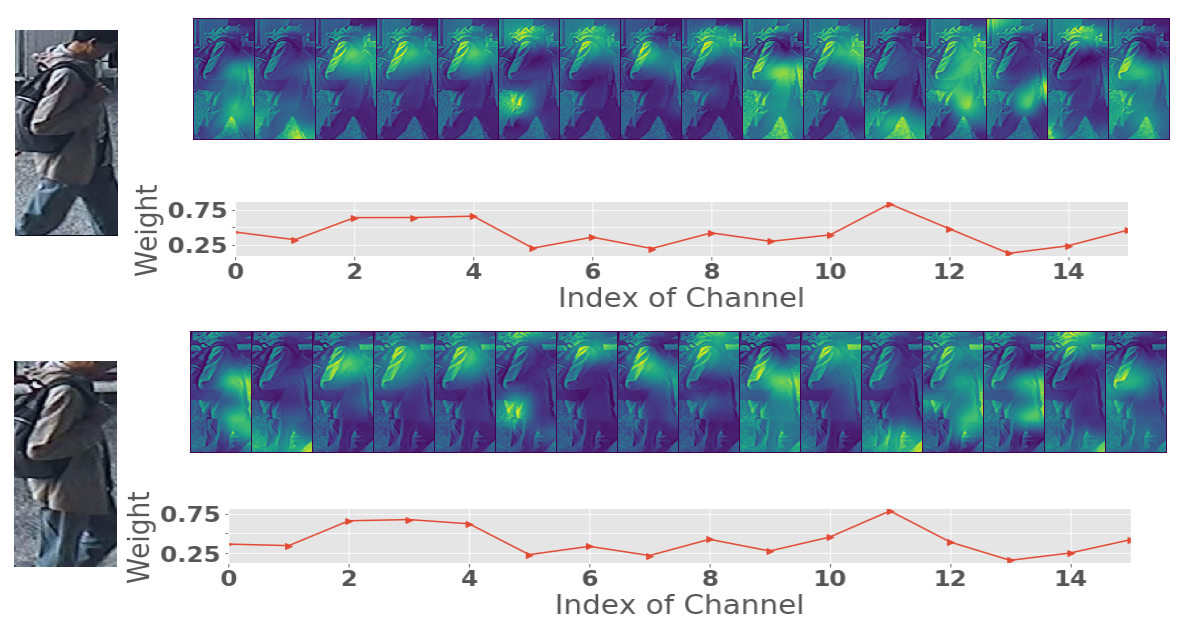
\includegraphics[width=\textwidth]{fig/comb2.png}
	\note{除去定量实验,还有定性实验,看不见的头部的注意力权重被降低}
\end{frame}

\begin{frame}{通道级别注意力}
	姿态变化
	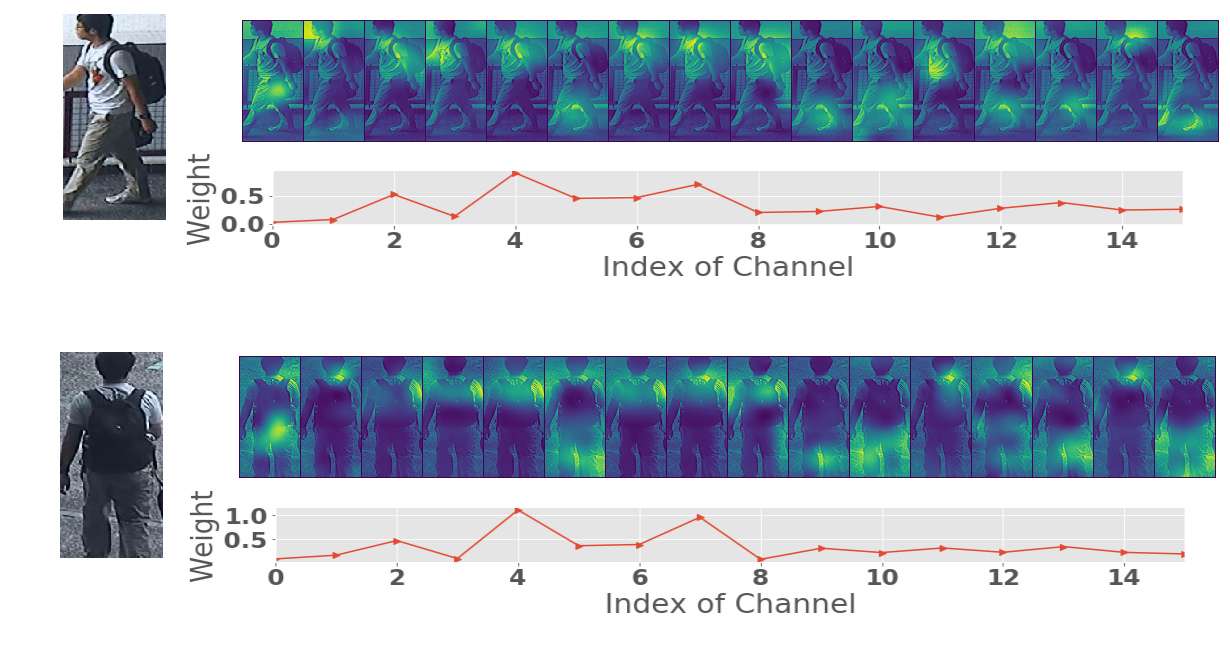
\includegraphics[width=\textwidth]{fig/comb1.png}
	\note{对姿态变化也具有鲁棒性,语义部件具有对应关系,看不见的腹部的权重被降低,头部、四肢具有对应关系,但是仍然还有缺点,就是因为行人的做肩膀和右肩膀很相似,所以我们的模型的左右不分,这一点之后也许可以引入一些上下文context信息来解决}
\end{frame}

\subsection{基于对比中心损失的度量学习}

\begin{frame}
	\frametitle{大纲}
	\tableofcontents[currentsection]
\end{frame}


\begin{frame}{动机:交叉熵的缺点}

	\begin{equation}
		\cL_{\textrm{Xent}} (\mX, \vtheta) = \sum_{j=1}^{N} \sum_{i=1}^{C}
		- y_{ji} \log \frac{\exp(\vw_i^T \vx_j)}{ \sum_{i=1}^C \exp(\vw_i^T \vx_j) }
	\end{equation}
\begin{columns}
\column{.55\textwidth} 
	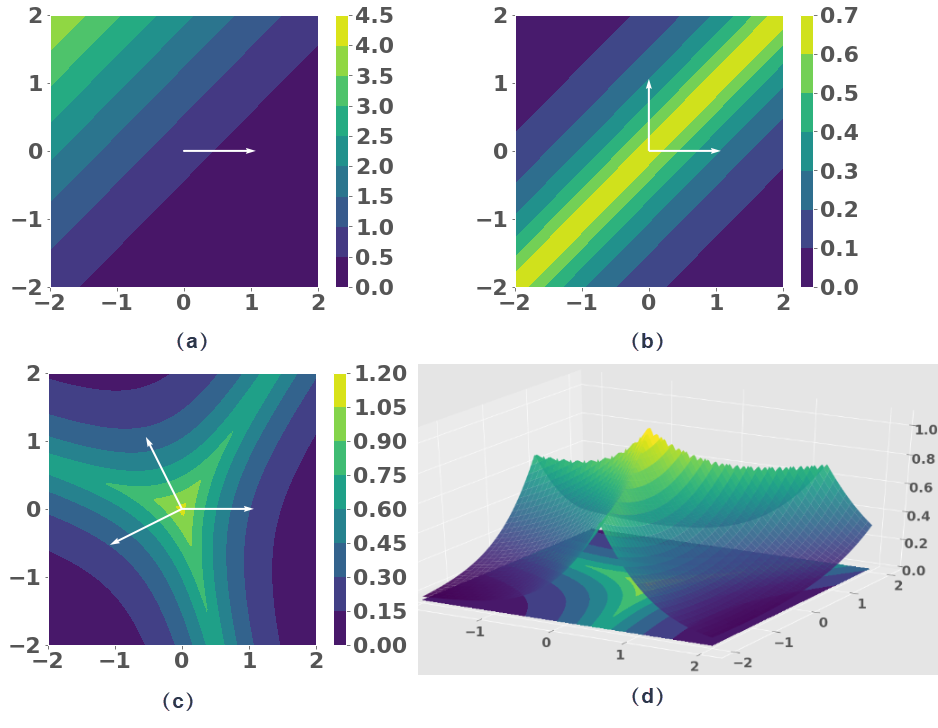
\includegraphics[width=\textwidth]{fig/xent.png}
	
\column{.45\textwidth} 
{\liuhao 
取$\vx=[x_1,x_2]^T$, 在二维上观察:\\ 
(a) 取
$
%\vw_1=[1,0]^T,\vw_2=[0,1]^T,
\mW= \begin{bmatrix}
1 & 0 \\ 
0& 1
\end{bmatrix}
$时, $-\log\frac{e^{x_1}}{e^{x_1}+e^{x_2}}$的等高线 \\
(b) $\min\{{-\log}\frac{e^{x_1}}{e^{x_1}+e^{x_2}}, -\log\frac{e^{x_2}}{e^{x_1}+e^{x_2}}\}$的等高线 \\
(c)  三分类, 取
$
%\vw_1=[1,0]^T,\vw_2=[-.5,1]^T,\vw_3=[-1,-.5]^T 
\mW= \begin{bmatrix}
1 & -.5 & -1 \\ 
0&1& -.5 
\end{bmatrix}$的等高线 \\
(d) 三分类时能量地形(loss landscape) 
}
\end{columns}

\note{我们知道输入图像首先会经过深度网络降为到特征空间 x ,首先来看损失函数会引导提取怎么样分布的特征。
结论是,交叉熵损失提取的特征的分布通常比较狭长, 比如

之后我们会有真实世界的数据来进一步验证 js 散度
}
\end{frame}

\begin{frame}{动机:难样本挖掘三元组损失的缺点}
Hermans \etal 提出TriHard: \cite{hermans2017defense}
	\begin{equation}
		\cL_{\textrm{TriHard}} (\mX, \vtheta) = \sum_{a=1}^{N} \max\left(
		0, m +
		{\color{NavyBlue}
		\max_{\substack{
				p=1...N \\
				y_a = y_p}
		} D(\vx_a, \vx_p) }
		-
		{ \color{Dandelion}
		\min_{ \substack{
				n=1...N \\
				y_a \neq y_n }
		} D(\vx_a,\vx_n) }
		\right)
	\end{equation}
	\begin{figure}
		\centering
		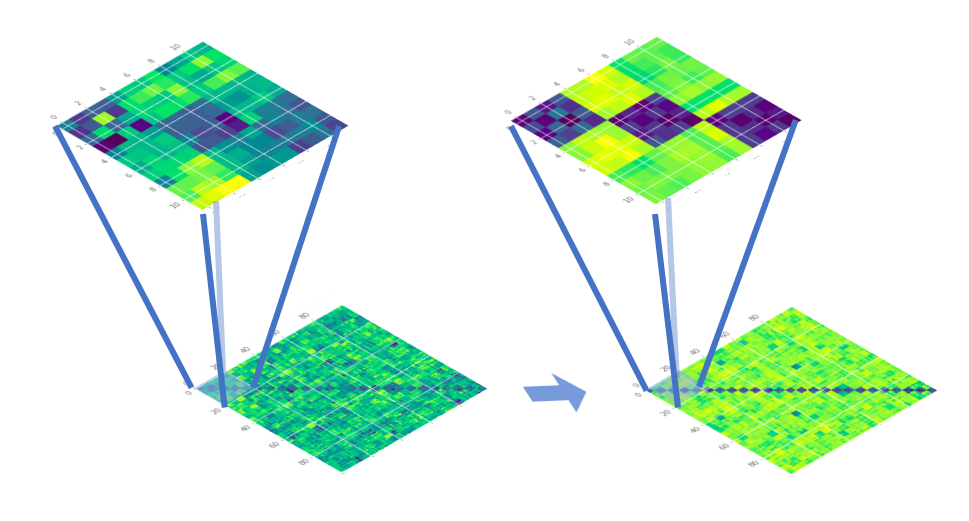
\includegraphics[width=.7\textwidth]{fig/2018-05-19-23-27-39.png}
		% \caption{从距离矩阵学习的角度理解难样本挖掘三元组损失} 
		\label{fig:distmat-tri}
	\end{figure}
	\note{SOA的代表}
\end{frame}

\begin{frame}{动机:特征的可分性与鉴别性}
	% 三种损失监督学习得到的
	\begin{columns}
		\column{.6\textwidth}
		\begin{figure}
			\centering
			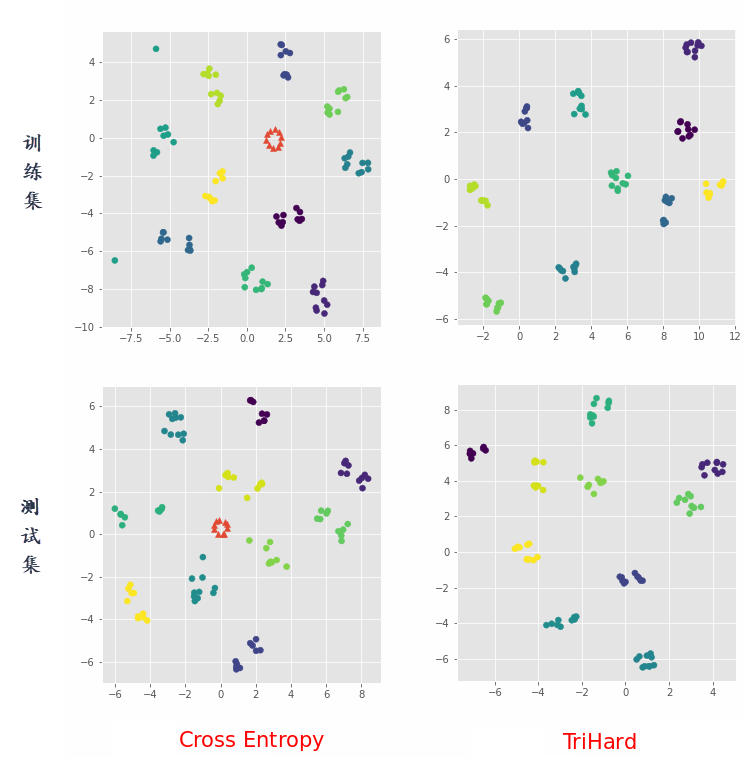
\includegraphics[width=\textwidth]{fig/final0.png}
			% \caption{三种损失函数监督的验证集特征向量和中心向量在2维平面上降维可视化,使用CUHK03数据集和各损失的基准模型得到}
		\end{figure}
		\column{.4\textwidth}
		\begin{itemize}
			\item 取10类行人的所有图片
			\item 使用收敛的模型提取128维特征向量
			\item T-SNE降维到2维可视化
		\end{itemize}
	\end{columns}
\end{frame}


\begin{frame}{动机:特征的可分性与鉴别性}
	% 三种损失监督学习得到的
	特征的可分性与鉴别性:
	\begin{figure}
		\centering
		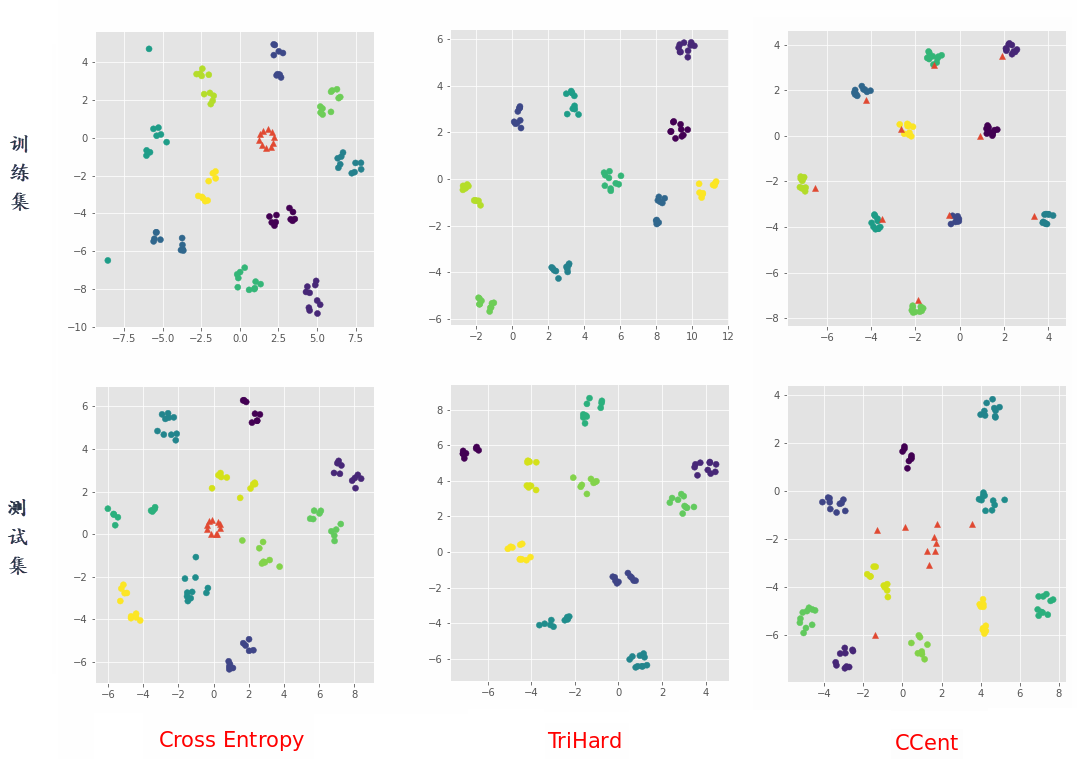
\includegraphics[width=.9\textwidth]{fig/final1.png}
		% \caption{三种损失函数监督的验证集特征向量和中心向量在2维平面上降维可视化,使用CUHK03数据集和各损失的基准模型得到}
	\end{figure}
\end{frame}


\begin{frame}{方案:与难样本三元损失对比}
	\begin{columns}
		\column{.5\textwidth}
		\begin{figure}
			\centering
			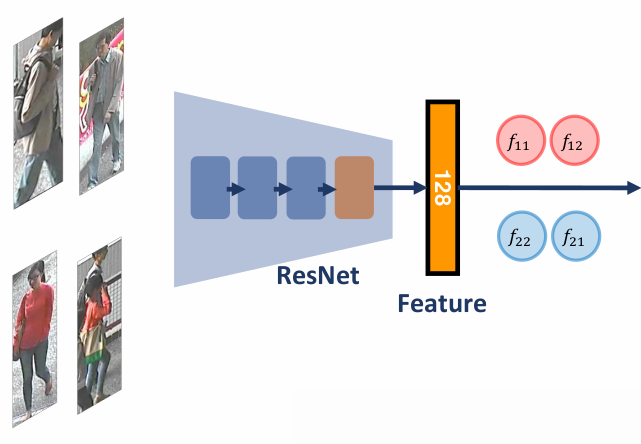
\includegraphics[width=\textwidth]{fig/over0.png}
			% \caption{
			% 	基于对比中心损失的行人再识别总体框图
			% }
			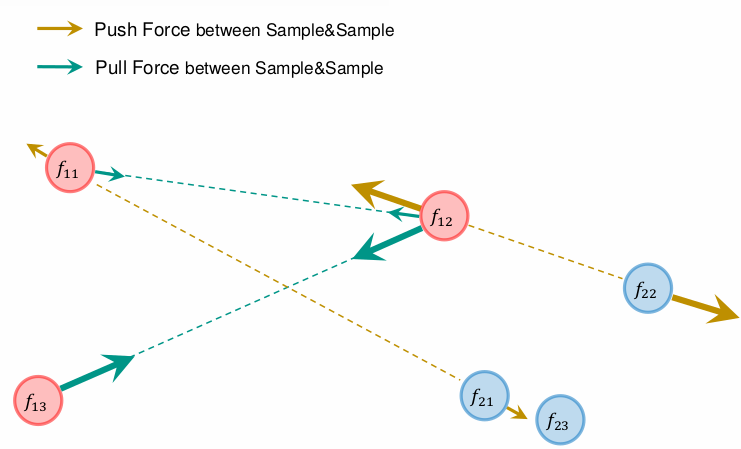
\includegraphics[width=\textwidth]{fig/illu0.png}
			% \caption{
			% 	\textbf{左图:}对比中心损失示意图;\textbf{右图:}难样本三元损失函数示意图
			% }
			\label{fig:dcent2}
		\end{figure}

		\column{.5\textwidth}

		\begin{figure}
			\centering
			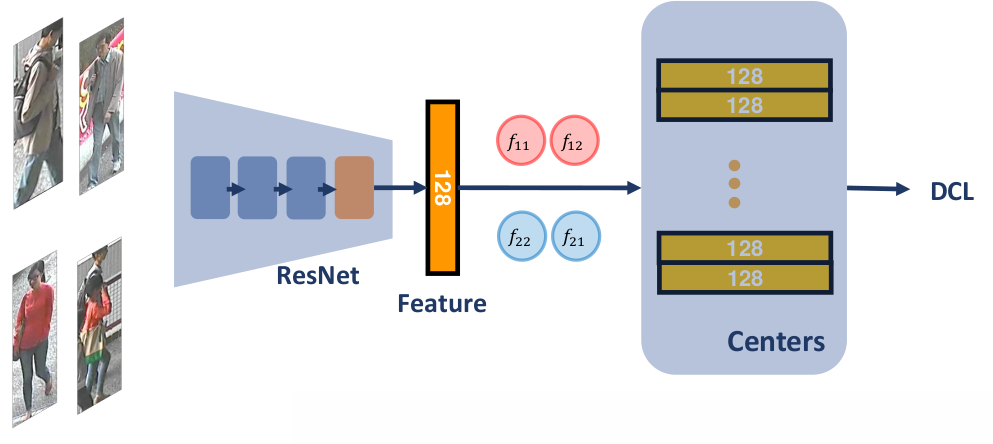
\includegraphics[width=\textwidth]{fig/over.png}
			% \caption{
			% 	基于对比中心损失的行人再识别总体框图
			% }
			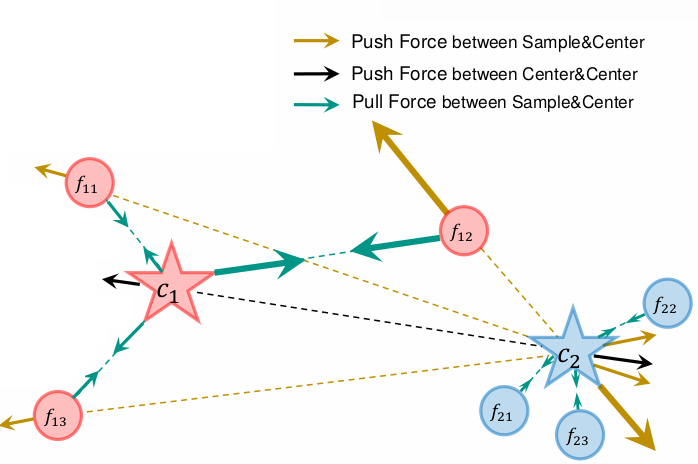
\includegraphics[width=\textwidth]{fig/illu1.png}
			% \caption{
			% 	\textbf{左图:}对比中心损失示意图;\textbf{右图:}难样本三元损失函数示意图
			% }
			% \label{fig:dcent2}
		\end{figure}
	\end{columns}

\end{frame}

\begin{frame}{方案:对比中心损失}
	\begin{equation*}
		\cL_{\textrm{CCent}} (\mX, \mC, \vtheta) = \frac{1}{2}
		\sum_{i=1}^{N}
		\frac{D(
			\vx_{i}, \vc_{y_i}
			)}{
			\displaystyle \lambda_s
			\min_{\substack{
					j=1...M \\
					j \neq y_i }}
			D(
			\vx_{i}, \vc_{j}
			) + 1 }
		-
		{	\color{Gray}
		\lambda_d \sum_{i=1}^{M}  \min_{j=1...M} D(\vc_i,\vc_j) }
		\label{eq:ccent}
	\end{equation*}
	\vspace{-1.5em}
	\begin{columns}
		\column{.5\textwidth}
		\begin{equation*}
			\begin{aligned}
				\pp{\cL_{\textrm{CCent}}}{\vx_i} & =
				{\color{ForestGreen}
				\frac{\vx_i -\vc_{y_i}}{\normsq{\vx_i - \vc_k } +1}
				}                                          \\
				                                 & \quad +
				{\color{BurntOrange}
				\frac{ ( \vc_k-\vx_i) \normsq{\vx_i - \vc_{y_i}}  }{\left[ \normsq{\vx_i - \vc_k } +1 \right]^2}
				}                                          \\
				\pp{\cL_{\textrm{CCent}}}{\vc_n} & =
				\sum_{i=1}^{N} \begin{cases}
					{\color{ForestGreen} \frac{\vc_{y_i} -\vx_i }{\normsq{\vx_i -\vc_k }+1} }                                        & ,y_i=n      \\
					{\color{BurntOrange}	\frac{(\vx_i - \vc_n)\normsq{\vx_i - \vc_{y_i}}}{ \left[\normsq{\vx_i - \vc_k}+1\right]^2 }} & ,y_i \neq n
				\end{cases}
			\end{aligned}
		\end{equation*}
		其中, $k=\displaystyle 
			\argmin_{\substack{
					j=1...M \\
					j \neq y_i }} D(\vx_i, \vc_j)$。
		\column{.5\textwidth}

		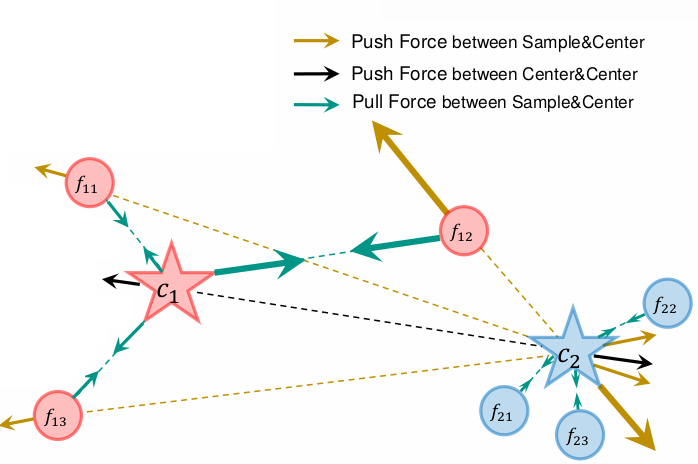
\includegraphics[width=\textwidth]{fig/illu1.png}
	
	\end{columns}
\end{frame}

\begin{frame}{优点}
	\begin{itemize}
		\item 鉴别性(更小的类内间距)+可分性
		\item 提高样本利用效率
		% \item 基本不增加计算量
		\item 多层次的损失,形成中心,便于全局挖掘
	\end{itemize}
\end{frame}

\begin{frame}{实验}
	在数据集CUHK03上的CMC-1,CMC-5,CMC-10性能指标比对:
	\begin{table}
		\centering
		% \caption{在数据集CUHK03上的CMC-1,CMC-5,CMC-10性能指标比对}
		\scalebox{0.9}{
			\begin{tabular}{c|ccc|ccc}
				\hline
				\multirow{2}*{Methods}                     &
				\multicolumn{3}{c|}{labelled CUHK03}       &
				\multicolumn{3}{c}{detected CUHK03}                                                                              \\
				\cline{2-7}
				\cline{2-7}
				                                           & r=1          & r=5     & r=10    & r=1          & r=5     & r=10    \\ \hline
				KISSME \cite{kissme}                       & 14.17        & 37.46   & 52.20   & 11.70        & 33.45   & 45.69   \\
				LMNN \cite{lmnn}                           & 7.29         & 19.64   & 30.74   & 6.25         & 17.87   & 26.60   \\
				LOMO+XQDA \cite{xqda}                      & 52.20        & 82.23   & 92.14   & 46.25        & 78.90   & 88.55   \\ \hline
				ImprovedDL \cite{improveddl}               & 54.74        & 86.50   & 93.88   & 44.96        & 76.01   & 81.85   \\
				DCSL (with hnm) \cite{yaqing2016semantics} & 80.20        & 97.73   & 99.17   & -            & -       & -       \\
				JLML \cite{jlml}                           & 83.20        & 98.00   & 99.40   & 80.60        & {96.90} & {98.70} \\
				SC-PPMN (with hnm) \cite{mao2018multi}     & {85.50}      & {98.20} & {99.50} & {80.63}      & 95.62   & 98.07   \\ \hline
				\hline
				Xent                                       & 76.93        & 95.16   & 97.76   & 71.67        & 91.36   & 95.34   \\
				+LblSmth                                   & 78.64        & 93.96   & 96.78   & 75.87        & 91.53   & 95.15   \\
				+Cent                                      & 82.21        & 95.55   & 98.39   & 80.12        & 95.38   & 98.11   \\
				% CCent                                      & 17.51   & 43.11   & 59.72   &         &         &         \\ 	 
				TriHard                                    & 84.50        & 98.49   & 99.24   & 82.48        & 97.15   & 98.38   \\
				+CCent                                     & \blue{87.77} & 98.70   & 99.55   & \blue{84.86} & 97.61   & 98.48   \\
				+CCent+Dis                                 & 88.12        & 98.80   & 99.40   & 84.45        & 97.15   & 98.44   \\   \hline
				% \hline
			\end{tabular}
		}
		\label{tab:cuhk032}
	\end{table}
\end{frame}

\begin{frame}{实验}
	在Market1501和DukeMTMC上的CMC-1, mAP性能指标对比:
	\begin{table}
		\centering
		% \caption{在数据集Market1501和DukeMTMC上的CMC-1, mAP性能指标对比}
		\label{tab:market2}
		\begin{tabular}{c|cc|cc}
			\hline
			\multirow{2}*{Method}                  & \multicolumn{2}{c|}{Market1501} & \multicolumn{2}{c}{DukeMTMC-ReID}                 \\
			\cline{2-5} \cline{2-5}                & r=1                             & mAP                               & r=1   & mAP   \\ \hline
			SomaNet \cite{zheng2017ped}            & 73.87                           & 47.89                             & 76.70 & 56.80 \\
			PAN \cite{barbosa2017looking}          & 82.81                           & 63.35                             & 71.59 & 51.51 \\
			TriHard in \cite{hermans2017defense}   & 82.99                           & 66.63                             & 73.24 & 54.60 \\
			AWTL        \cite{ristani2018features} & 84.20                           & 68.03                             & 74.23 & 54.97 \\ \hline  \hline
			Xent                                   & 84.92                           & 65.15                             & 72.44 & 51.16 \\
			+LblSmth                               & 89.46                           & 72.18                             & 79.08 & 59.80 \\
			+Cent                                  & 82.42                           & 61.77                             & 73.81 & 53.29 \\
			TriHard                                & 86.55                           & 69.98                             & 75.08 & 57.10 \\
			+CCent                                 & \blue{89.12}                    & 71.57                             & 81.54 & 62.33 \\
			+CCent+Dis                             & 90.37                           & 72.94                             & 80.36 & 60.87 \\  \hline
		\end{tabular}
	\end{table}
\end{frame}

\section{思考与展望}

\begin{frame}{思考与展望}
	\begin{itemize}
		\item 基于注意力机制的多尺度特征融合
		\begin{itemize}
			\item 有选择地提取属性特征
			\item 解耦和重标定语义部件
		\end{itemize}
		\item 基于对比中心损失的度量学习
		\begin{itemize}
			\item 鉴别性(更小的类内间距) + 可分性
			\item 多层次的损失,形成中心,便于全局挖掘
		\end{itemize}
	\item 展望
	\begin{itemize}
		\item 对抗噪声、鲁棒性与可解释性
		\item 上下文信息
		\item 伪三维注意力
		\item 不变性与同变形
	\end{itemize}
	\end{itemize}
	 \note{
		 % todo read senet 
		 % todo read f-gan --> xent js div
	 }
\end{frame}

\begin{frame}
	\chuhao Thank you! %\fontspec{LHANDW.TTF}
\end{frame}

\section{附录}

\begin{frame}[t, allowframebreaks]
\frametitle{参考文献}
\printbibliography
\end{frame}

\begin{frame}{贡献}
\url{https://github.com/KaiyangZhou/deep-person-reid}
		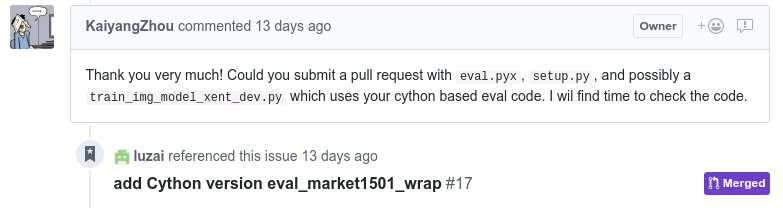
\includegraphics[width=\textwidth]{fig/2018-06-01-12-19-14.png}
	\url{	https://github.com/bearpaw/pytorch-classification}
		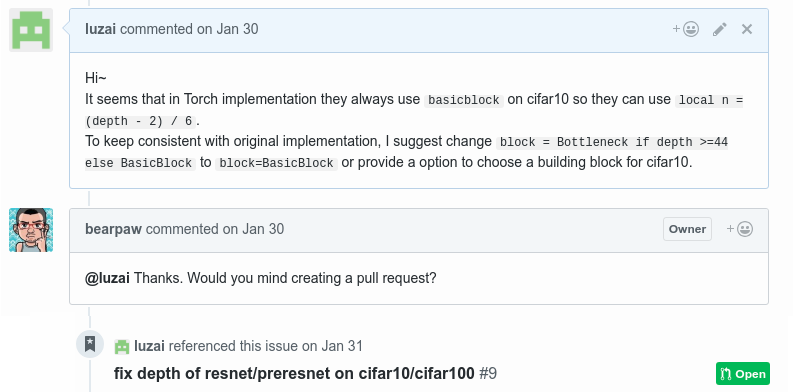
\includegraphics[width=\textwidth]{fig/2018-06-01-12-19-39.png}
\end{frame}


\begin{frame}{显著性与可解释性}
	\begin{figure}
		\centering
		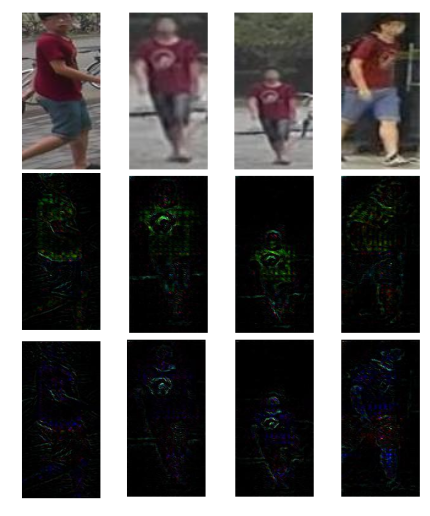
\includegraphics[width=.47\textwidth]{2018-05-21-09-58-23.png}
		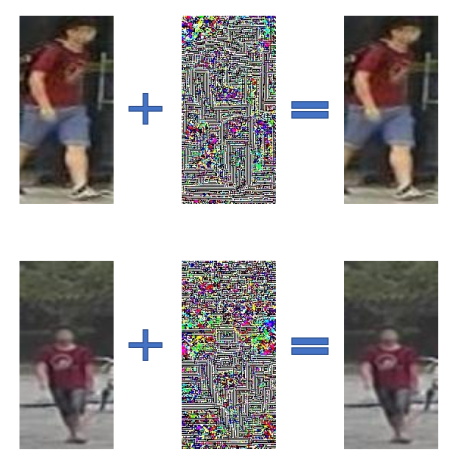
\includegraphics[width=.47\textwidth]{2018-05-21-10-31-13.png}
	\end{figure}

\end{frame}

\begin{frame}
{WGAN}
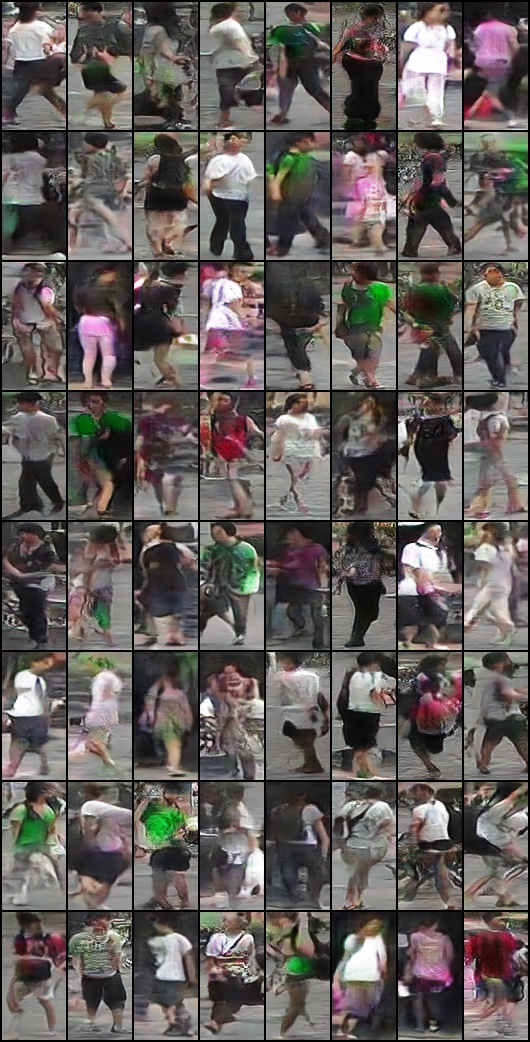
\includegraphics[height=\textheight]{wgan0.png}
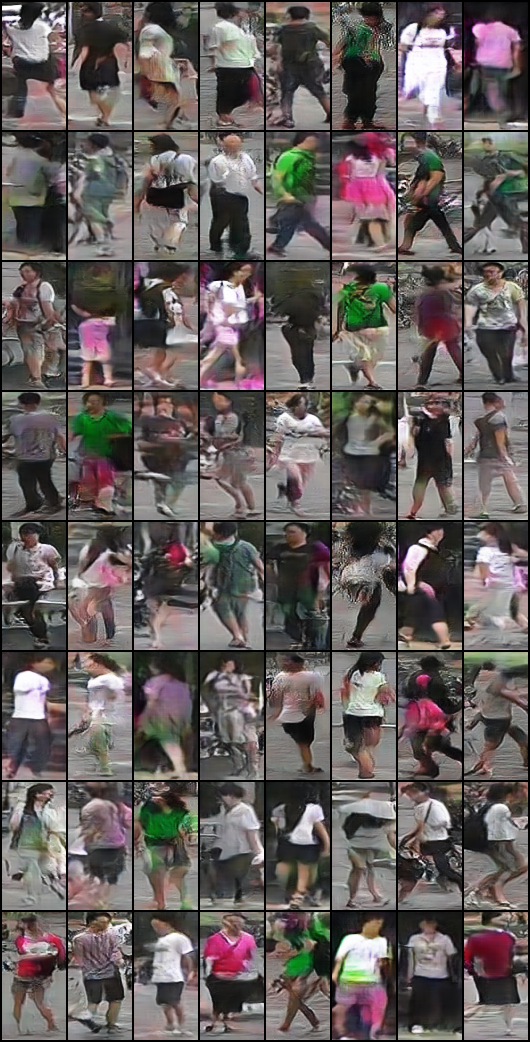
\includegraphics[height=\textheight]{wgan1.png}

\end{frame}

\begin{frame}{项目日志}
\url{https://luzai.github.io/report}  \\
\url{http://10.13.72.84:8000} \\ 
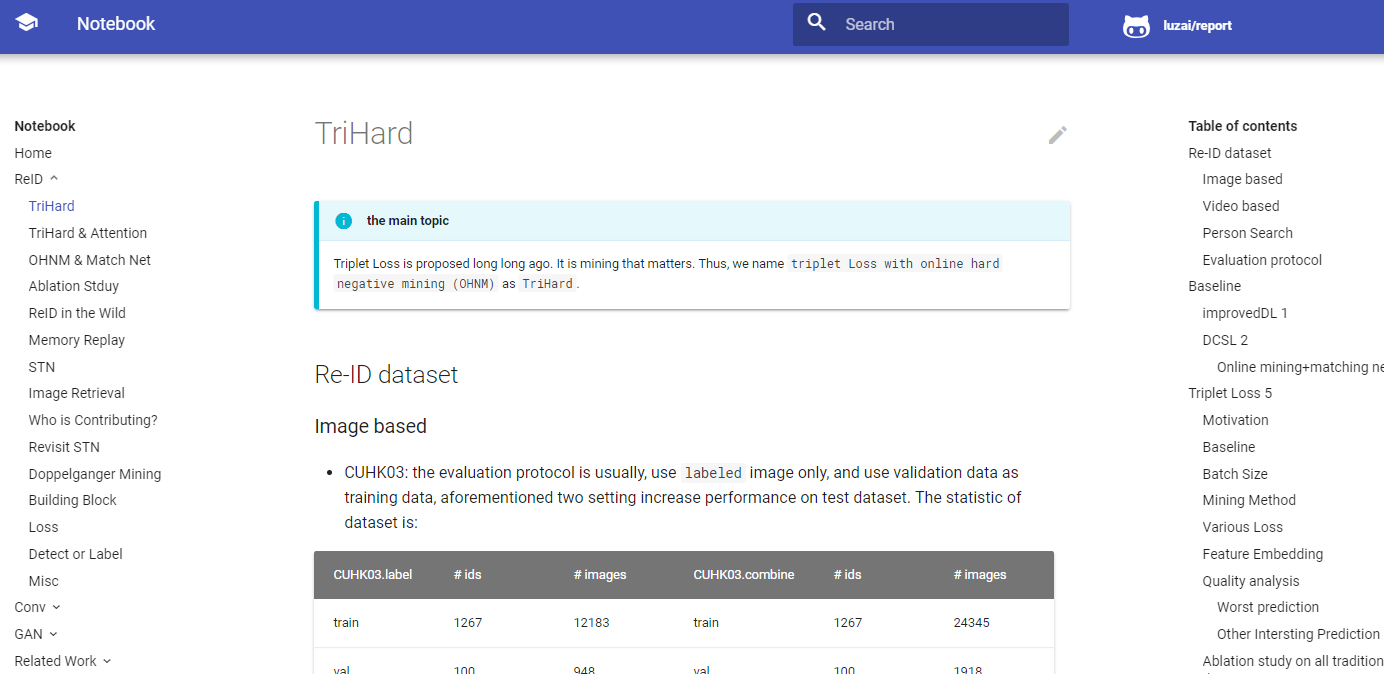
\includegraphics[width=\textwidth]{fig/ref.png}
\end{frame}

\begin{frame}{维度诅咒}
\begin{figure}
	\centering
	\includegraphics[width=\textwidth]{dim-curse.png}
\end{figure}
\end{frame}
\begin{frame}{不变性与同变性}
	\begin{figure}
		\centering
		\includegraphics[width=.75\textwidth]{2018-05-21-10-51-51.png}
	\end{figure}
\end{frame}
\begin{frame}[fragile]
	\frametitle{eval protocol}
	\begin{lstlisting}
cmc_configs = {
'cuhk03': dict(separate_camera_set=True,
  single_gallery_shot=True,
  first_match_break=False),
'market1501': dict(separate_camera_set=False,#h
  single_gallery_shot=False,  # hard
  first_match_break=True),
'allshots': dict(separate_camera_set=False,#h
  single_gallery_shot=False,  # hard
  first_match_break=False),
}
\end{lstlisting}
\end{frame}

\end{document}
